This section outlines benchmark models for both Quantum Chromodynamics (\QCD)~and for new
physics signals and is taken directly from \cite{Bauce:2226443}. These are used in the search and limit-setting phases of the
analysis and for testing the effects of potential
resonant and non-resonant signals on the search phase.
The main characteristics of resonant and non-resonant
signals are encapsulated in the models chosen:
excited quarks (\qstar{}), quantum black holes (\QBH), 
a \Wprime\ signal with decays to quarks,
\Zprime\ signals consist with recent recommendations from the 
ATLAS-CMS Dark Matter Forum~\cite{Abercrombie:2015wmb},
a \Wstar\ signal with decays to quarks,
and non-resonant contact interactions (\CI).

Samples reconstructed with release 21.2 are used for 2015 and 2016 data as well as for Monte Carlo. EXOT2 skimmed samples, described in~\cite{ATLAS:Exot2Derivation}, are used in this analysis.

\subsection{Quantum Chromodynamics}
\label{qcdsamps}
\QCD processes from the SM are simulated at leading order (\LO)
and next-to-leading order (\NLO) in perturbative \QCD. 
%Table~\ref{tab:qcdSamps} gives the details on the \QCD~MC used.

In order to obtain a \NLO~prediction from \Pythia~events, they are reweighted to the 
predictions of NLOJET++ (\NLO~$K$-factors) and subsequently by Electroweak (EW) $\kappa$~factors. 
These $K$-factors and $\kappa$~factors are binned in \mjj\ and $\chi$; full details are given in Sec.~\ref{sec:ang_bkgd}.  The \NLO\ corrected
version of \Pythia8 is used for the statistical comparison of the 
data to the background for the angular analysis.

\QCD samples span such a large range in cross section that the
production must be split in order to obtain comparable statistical precision
across the kinematic range of interest.
The well established procedure of dividing \QCD~production according
to the leading jet \pT~and reweighting the underlying spectrum
is described in Ref.~\cite{Marshall:2016630}.  

\subsection{Resonant Models}
\subsubsection{Excited quarks}
\label{sec:qstar}

Excited quark (\qstar) production and subsequent decay to
quarks and gluons via gauge interactions has been
used as a common benchmark for the dijet mass resonance
search~\cite{EXOT-2010-01,EXOT-2010-02,EXOT-2010-07,EXOT-2011-07,EXOT-2013-11,EXOT-2016-21},
and it is described in detail in Refs~\cite{Baur:1987ga,Baur:1989kv}.
The $qg\to$ \qstar production model~\cite{Baur:1987ga,Baur:1989kv} is used,
with the assumption of spin 1/2 and quark-like SM coupling constants.
The compositeness scale ($\Lambda$) is set to the \qstar~mass.

The excited quark signal templates are generated for different mass values
(Table~\ref{tab:qStarSamps}) with the \Pythia~8 event generator~\cite{pythia8},
using the A14 tune~\cite{A14tune} and NNPDF2.3 PDF set~\cite{Carrazza:2013axa}. Both light flavor ($u$,$d$,$s$) and heavy flavor ($c$,$b$) quarks are taken into account in
the event generation.
After a basic selection, no duplicate events have been identified.
All samples are fully simulated using \Geant.


Figures~\ref{fig:signal_xsec} and~\ref{fig:acc} show the cross sections and
acceptances as a function of the signal mass point.  
The acceptance shown for the \qstar model for 13~\TeV~center-of-mass energies 
uses the full resonance analysis selection (Section~\ref{sec:event_selection}).
The interpolation between points is a straight line therefore the
acceptance between m=1~\TeV~and m=2~\TeV~is not an accurate representation
of what the acceptance of a m=1.5~\TeV~sample would be.  The
interpolation is not used but drawn to help guide the eye.

\begin{figure}[!htb]
  \centering
  \subfigure[Cross section]{ \label{fig:signal_xsec} 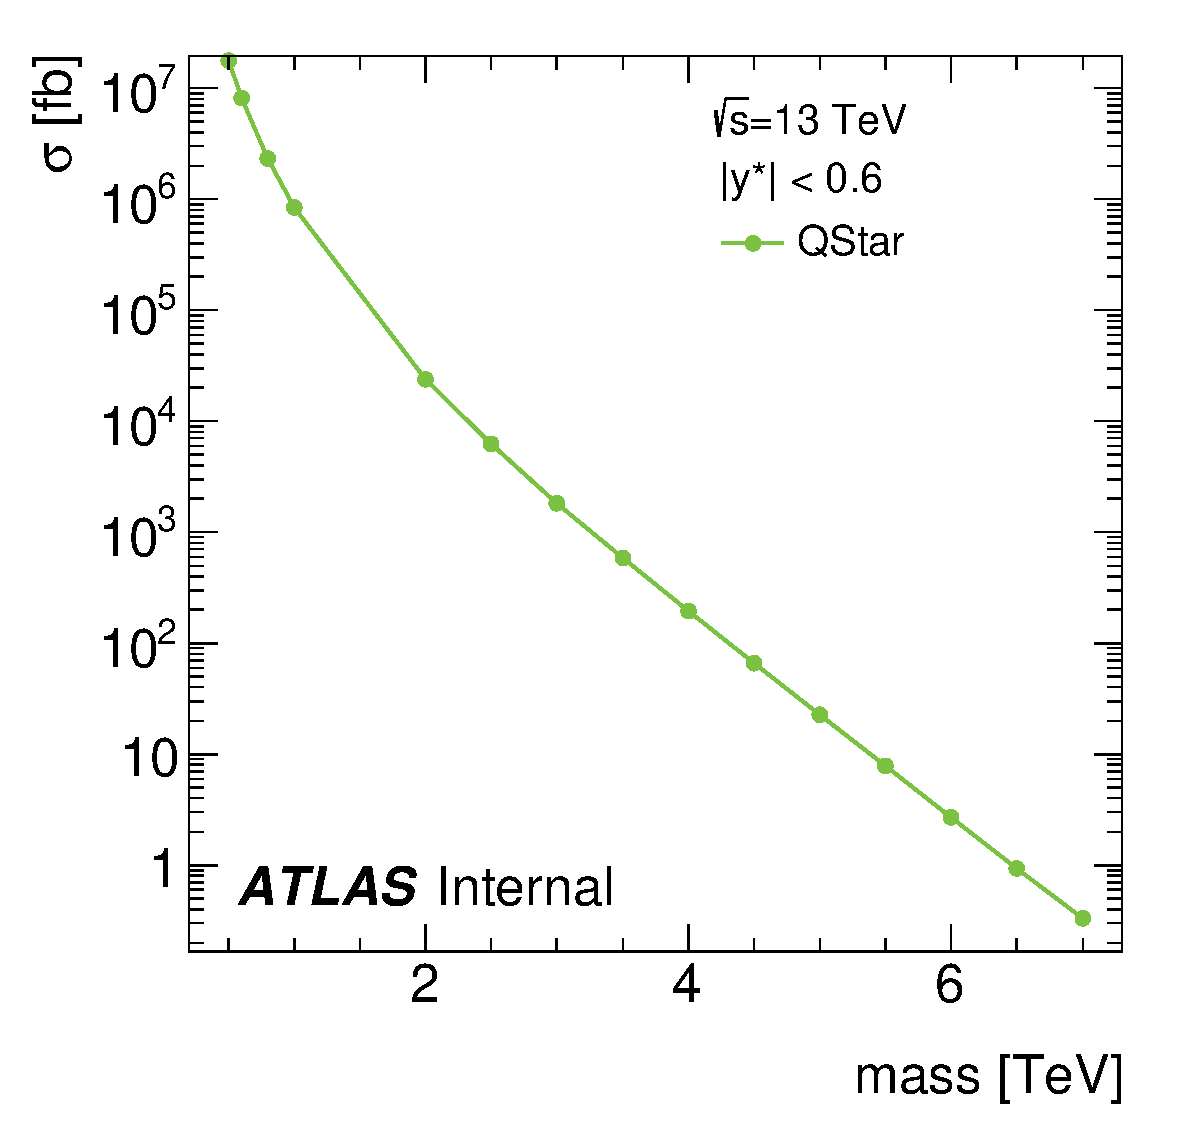
\includegraphics[width=0.48\textwidth]{figures/benchmark_signals/CrossSections_QStar_log} }
  \subfigure[Acceptance]{ \label{fig:acc} 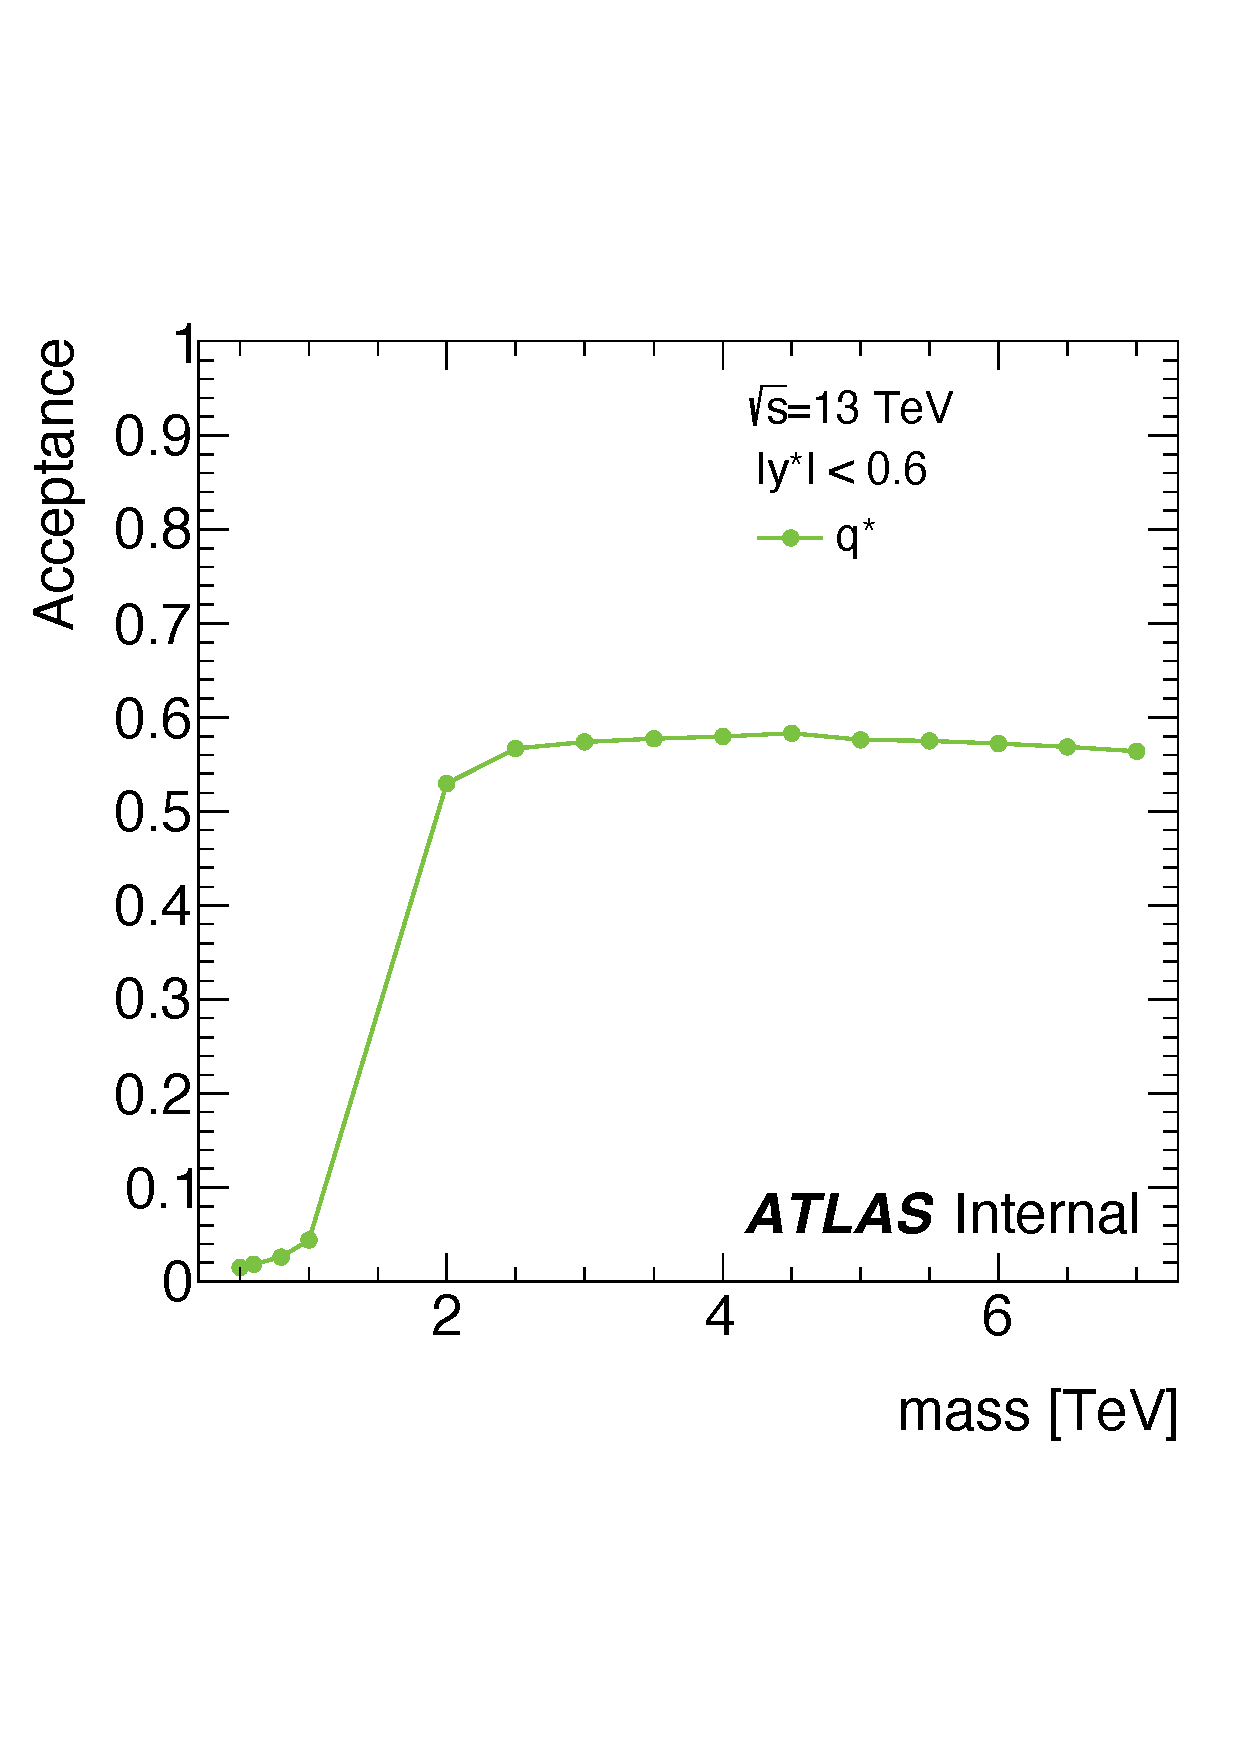
\includegraphics[width=0.48\textwidth]{figures/benchmark_signals/Acceptances_QStar} }
  \caption{(a) Cross section and (b) acceptance for the 
  light-flavored \qstar model for 13~\TeV~center-of-mass energies using the full resonance
  analysis selection (Section~\ref{sec:event_selection}).}
\end{figure}


\clearpage

%\subsubsection{Quantum Black Holes}
%\label{sec:QBH}
%\todo{Do QBH decay to quarks or gluons, is there increased sensitivity or not} 
%The LHC should be able to produce QBH under the condition that the
%universe contains sufficiently large extra dimensions \cite{RandallMeade}.
%The quantum-gravity energy scale $M_{D}$ at which micro black holes are produced decreases as the number, $n$,
%of these large extra dimensions increases, allowing for lower mass scales at larger $n$.
%
%In the simplest situation, one would expect approximately isotropic decay of these micro black holes via Hawking
%radiation to a many-particle final state. This would require black holes (BH) to be produced substantially
%above their mass threshold in order to have energy for such a decay \cite{Feng:2004}. 
%However, gravitational interactions are also expected at the scale of the new interaction 
%(well below the actual thermal black hole production threshold), at which the dominant final state would be two-body ones.
%Production of these
%states is expected to begin once the $M_D$ energy threshold is reached. 
%This results in a resonance-like production of predominantly
%two-body final states, mainly jets, near $M_D$. The dijet analysis, then, is a way to search for such
%isotropic final states as probes of quantum gravitational effects.
%
%The \BlackMax~\cite{Dai:2007ki} MC generator is used to simulate quantum black holes events with $n=6$. The samples used in the analysis
%are listed in Table~\ref{tab:qbhSamps}. Cross sections and acceptances for the model are given in figures~\ref{fig:signal_xsec_blackmax} and~\ref{fig:acc_blackmax} respectively.
%
%\begin{figure}[!htb]
%  \centering
%  \subfigure[Cross section]{\label{fig:signal_xsec_blackmax} 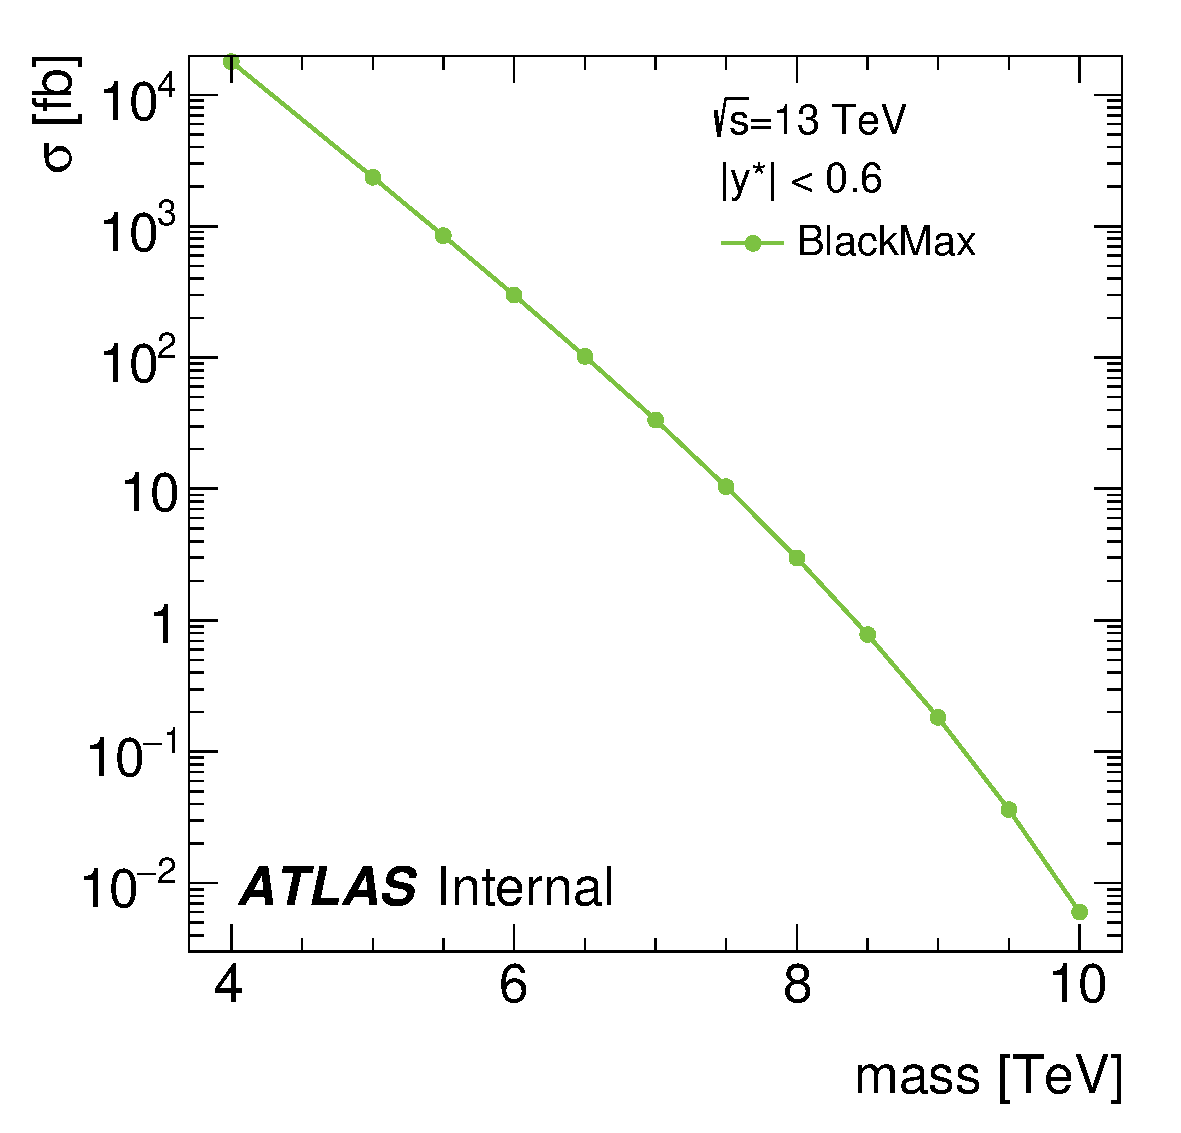
\includegraphics[width=0.48\textwidth]{figures/benchmark_signals/CrossSections_BlackMax_log}}
%  \subfigure[Acceptance]{  \label{fig:acc_blackmax}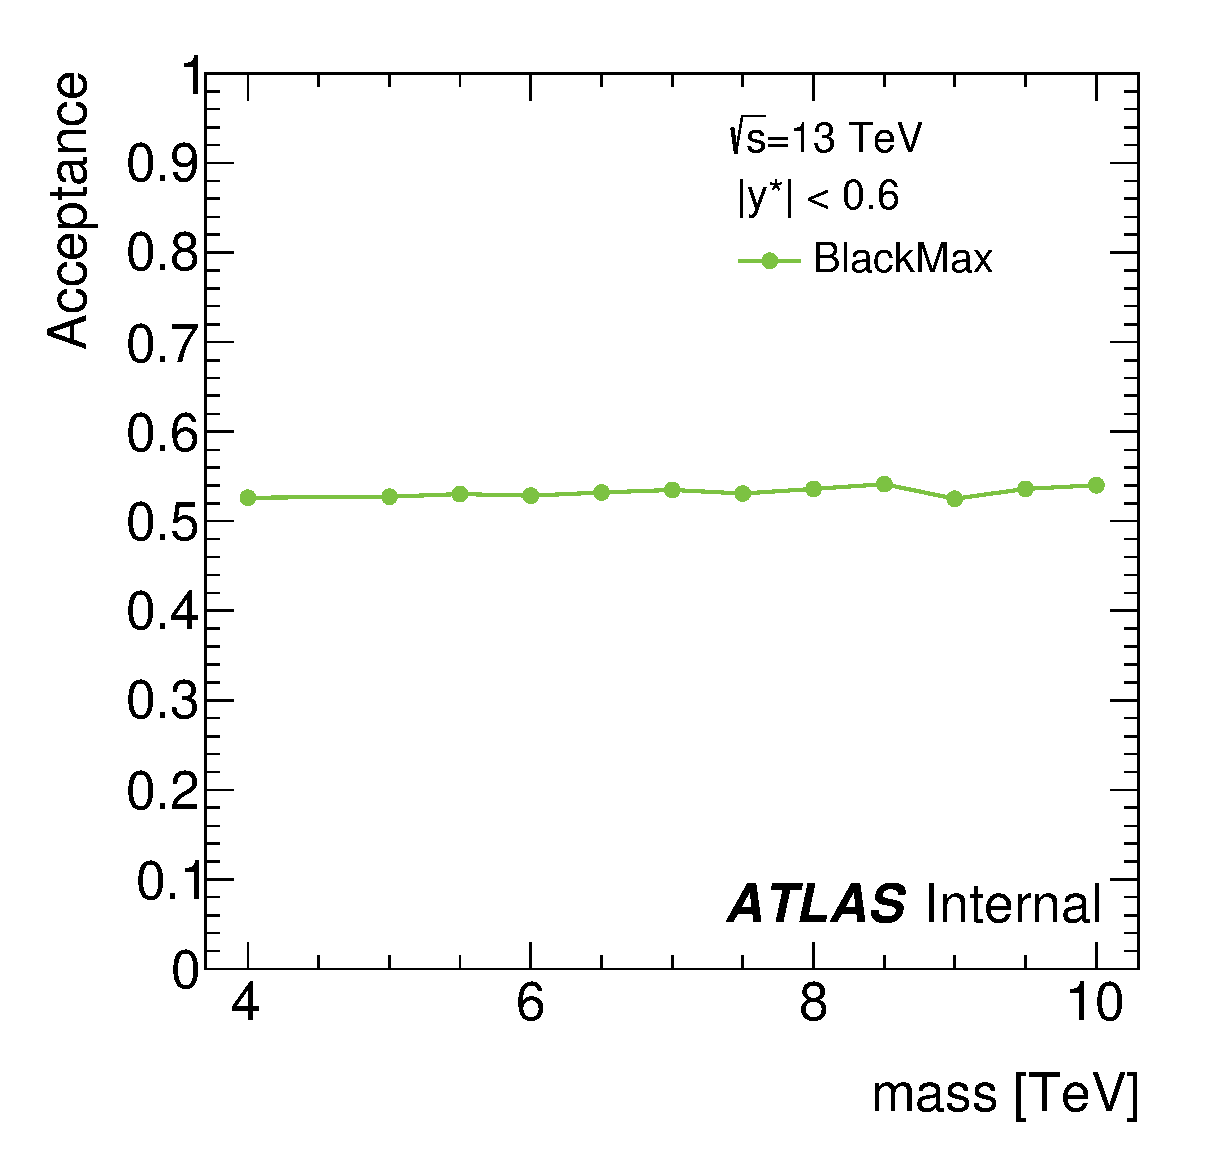
\includegraphics[width=0.48\textwidth]{figures/benchmark_signals/Acceptances_BlackMax}}
%  \caption{(a) Cross section and (b) acceptance for the 
%  \BlackMax\ model for 13~\TeV~center-of-mass energies using the full resonance
%  analysis selection (Section~\ref{sec:event_selection}).}
%
%\end{figure}
%
%
%
%\clearpage

\subsubsection{\Zprime\ models}
\label{sec:Zprime}

Searches for dijet resonances play an important role in constraining
possible interactions between dark matter, or a "dark sector," and the
Standard Model. In this analysis, we consider the pure axial-vector
leptophobic \Zprime\ model described by the ATLAS-CMS Dark Matter Forum
Report \cite{Abercrombie:2015wmb}, in the specific scenario outlined in Ref.\cite{Chala:2015ama}, 
where dijet searches complement mono-jet-like searches in regions of
parameter space where the decay of the \Zprime\ to invisible particles is
kinetically suppressed. Regions of the parameter space of this model
remain which can be probed by dijet resonance searches but LUX, relic
density constraints, and monojet searches cannot constrain.
% 
In this model, the \Zprime\ arises from a simple extension of the Standard
Model (SM) with an additional $U(1)$ gauge symmetry and a Dirac
fermion Dark Matter particle that has charges only under this new
group. Assuming that some SM particles are also charged under this
group, the \Zprime\ can mediate interactions between the SM and DM. The DM
particle $\chi$ has a mass $m_{DM}$. The spin-1 \Zprime\ has mass \mMed.

The Dark Matter Forum reports models with vector or axial-vector couplings
between the spin-1 mediator $\Zprime$ and SM and DM fields, with the corresponding interaction Lagrangians:

\begin{align}
	\label{eq:AV}
	\mathcal{L}_{\mathrm{vector}} &= \gq \sum_{q={u,d,s,c,b,t}}  \Zprime_{\mu} \bar{q}\gamma^{\mu}q + \gDM \Zprime_{\mu} \bar{\chiDM}\gamma^{\mu}\chiDM \\
	\mathcal{L}_{\mathrm{axial-vector}} &= \gq \sum_{q={u,d,s,c,b,t}}  \Zprime_{\mu} \bar{q}\gamma^{\mu}\gamma^5q + \gDM \Zprime_{\mu} \bar{\chiDM}\gamma^{\mu}\gamma^5\chiDM.
\end{align}

The parameters in the model are thus
\begin{equation}
\left\{~\gq, 
~ \gDM, 
~\mDM,
~\mMed,
\right\} \,.
\end{equation}

where ~\gq is the coupling of the \Zprime\ mediator to quarks, ~ \gDM
is its coupling to the Dark Matter fermion, ~\mDM is the mass
of the Dark Matter fermion and~\mMed is the \Zprime\ mass. 

The two most relevant parameters of this model in the dijet search are the coupling of the \Zprime\ to quarks
as it drives the intrinsic width of the resonance, and the \Zprime\ mass. 
These two parameters are scanned to obtain the signal grid used
for the limit setting. The Dark Matter mass is fixed at 10 TeV and the coupling to DM to 1.5, with 
a negligible effect on the resonance width. 
% 
The values of $\gq$ and $\mMed$ have been kept consistent with the previous published dijet result.
The requested $\mMed$ points only go up to 3.5~TeV. This is where the resonance reaches the maximum width
that this search is sensitive to, without incurring in significant background distortion. 
For wider signals, it would be necessary to account for interference with the standard model.

The grid of samples produced in full simulation is shown in Table~\ref{tab:ZPrimeScan}.

\begin{table}[!h]
	\centering
		\begin{tabular}{| l |r r r r r r r r r r|}
			\hline
			\multicolumn{1}{|c|}{\mMed/\gev} & \multicolumn{10}{c|}{\gq} \\
			\hline
			1500   	       &         0.1  & 0.2 & 0.3 &  &  &  &  &  &  &  \\
			2000           &         0.1  & 0.2 & 0.3 & 0.4  &  &  &  &  &  &  \\
			2500           &         0.1  & 0.2 & 0.3 & 0.4 & 0.5 &  &  &  &  &  \\
			3000           &         0.1  & 0.2 & 0.3 & 0.4 & 0.5 &  &  &  &  &  \\
			3500           &         0.1  & 0.2 & 0.3 & 0.4 & 0.5 &  &  &  &  &  \\
			\hline
		\end{tabular}
%	}
	\caption{Parameter grid in \gq and \mMed scanned in full simulation with 25 ns configuration.}.
	\label{tab:ZPrimeScan}
\end{table}
 
 The acceptances %and cross-sections 
 for the \Zprime\ samples
 are shown in Figure~\ref{fig:zprime_acc}.% and \ref{fig:zprime_xsec} respectively. 

 \begin{figure}[!htb]
   \centering
   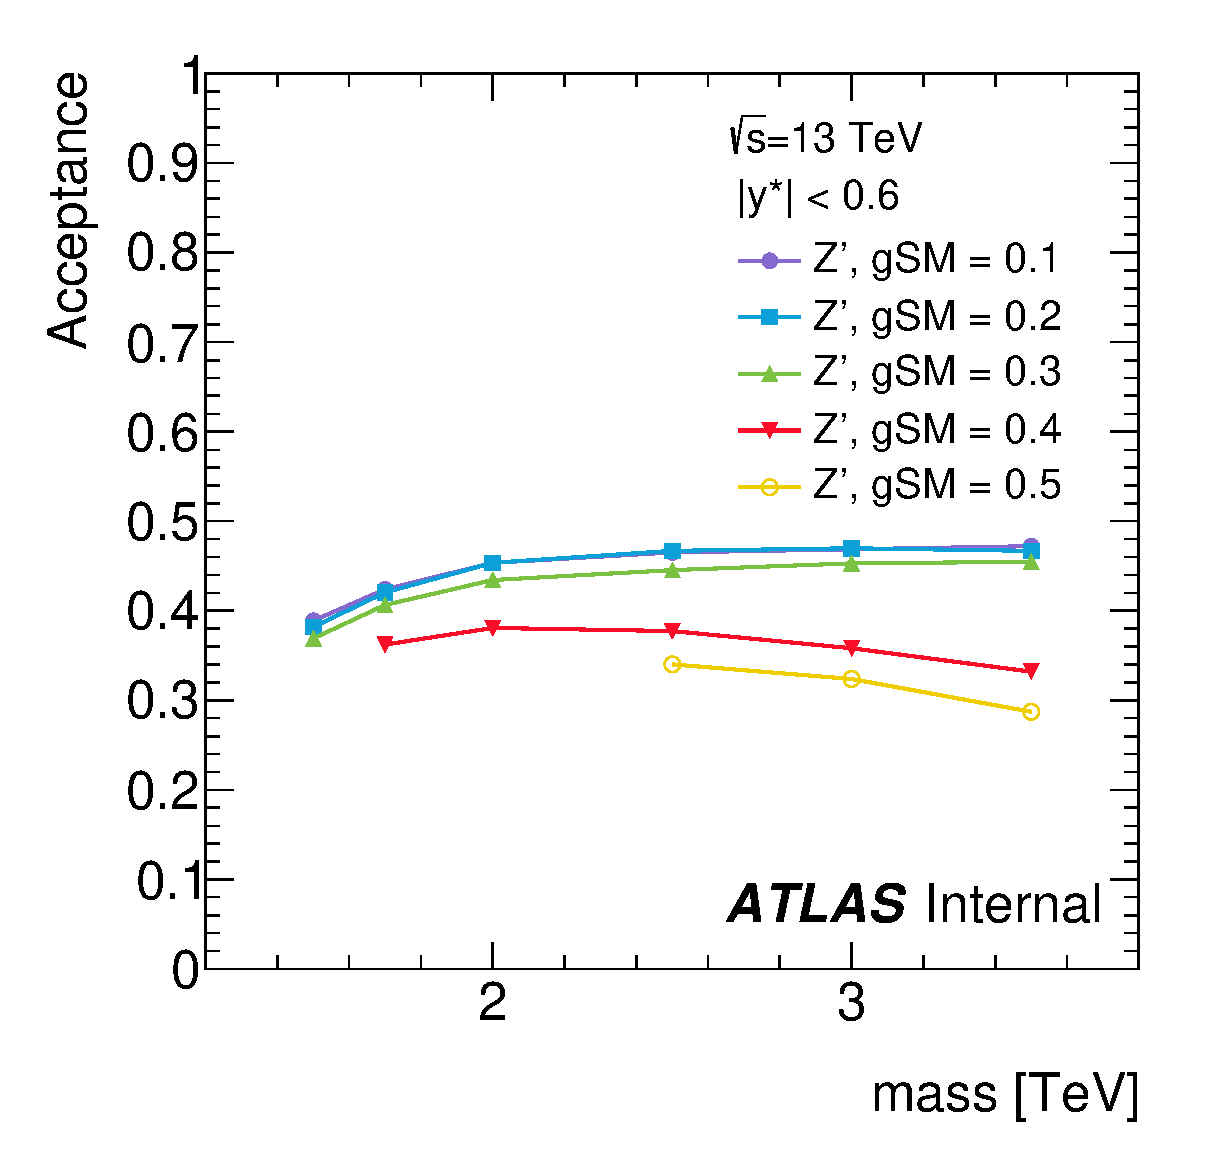
\includegraphics[width=0.45\textwidth]{figures/benchmark_signals/Acceptances_AllZPrime.eps}
   \caption{Acceptance for the \Zprime\ models 
   for 13~\TeV~center-of-mass energies using the full resonance
   analysis selection (Section~\ref{sec:event_selection}).
   \label{fig:zprime_acc}}
 \end{figure}
 
 \clearpage
\subsubsection{\Wstar\ Model}
\label{sec:Wstar}

 A search has been performed for a \Wstar, a chiral excitations of the W boson, described in \cite{Chizhov:2010jg}, with further theoretical motivation in \cite{Chizhov:2009fc}. The presence of such an excited boson could be the evidence of W-boson compositeness. These excitations would couple to $qg$ final states and would lead to resonances in the dijet invariant mass spectrum. Their angular distributions would differ strongly from those of all other models considered here, with a $cos^{2}\theta$ dependence that produces an excess focused more towards the forward region. 

 A simplified model \cite{Chizhov:2010ry}, with the Lagrangian available in the CalcHEP 3.6 generator, has been utilised in the current studies. Using the NNPDF23$\_$nlo PDF, \Wstar event samples have been generated for masses ranging from 1.8 TeV to 4.0 TeV in steps of 200 GeV, which are then passed to Pythia8 for hadronisation. 

The Langrangian of this Model is shown in equation (\ref{L}) where $\sin \theta_{X}$ is the mixing angle.

\begin{eqnarray}\label{L}
{\cal L}_{ref}&=&\frac{g}{\sqrt{2}M_{Z^*_d}}\left(
\bar{d}\sigma^{\mu\nu}d+\bar{e}\sigma^{\mu\nu}e
\right)\partial_\mu Z^*_{d\nu}+
\frac{\sqrt{2}g}{\sqrt{3}M_{Z^*_u}}\left(\bar{u}\sigma^{\mu\nu}\!u\;
\partial_\mu {\mathrm Re}Z^*_{u\nu}+
i\,\bar{u}\sigma^{\mu\nu}\gamma^5\!u\;
\partial_\mu {\mathrm Im}Z^*_{u\nu}\right) \nonumber\\
&&\hspace{-0.8cm}+\frac{g}{M_{W^*}}\left(\sin\theta_X\,\overline{u_L}\sigma^{\mu\nu}d_R+
\frac{2}{\sqrt{3}}\cos\theta_X\,\overline{u_R}\sigma^{\mu\nu}d_L+
\sin\theta_X\,\overline{\nu_L}\sigma^{\mu\nu}e_R
\right)\partial_\mu W^{*+}_{X\nu} + {\mathrm h.c.},
\end{eqnarray}

\Wstar\ samples can be generated using two different mixing angles.
\begin{itemize}
\label{sec:WstarSamples}
\item Using mixing angle ($\sin \theta_X$) = 1 which favours leptonic decay. This leads to lower senstivity to dijet channel but can be used to compare the results with di-lepton final states.
\item Using mixing angle ($\sin \theta_X$) = 0 which is lepto-phobic and favours jets as a final state. The advantage of using this condition is to have increase in sensitivity of the search  in dijet final states. 
\end{itemize}

\Wstar\ states were generated with lepto-phobic mixing angle ($\sin \theta_X$)=0 in this study because of the higher sensitivity of dijet final states in these models.


Figures~\ref{fig:Wstar_xsec} and~\ref{fig:Wstar_acc} show the cross sections and
acceptances as a function of the signal mass point.  
The acceptance shown for the \Wstar\ model for 13 TeV~center-of-mass energies 
uses the full resonance analysis selection for \Wstar\ signal (Section~\ref{sec:event_selection} where |y*|<1.2).

\begin{figure}[!htb]
  \centering
  \subfigure[Cross section]{\label{fig:Wstar_xsec}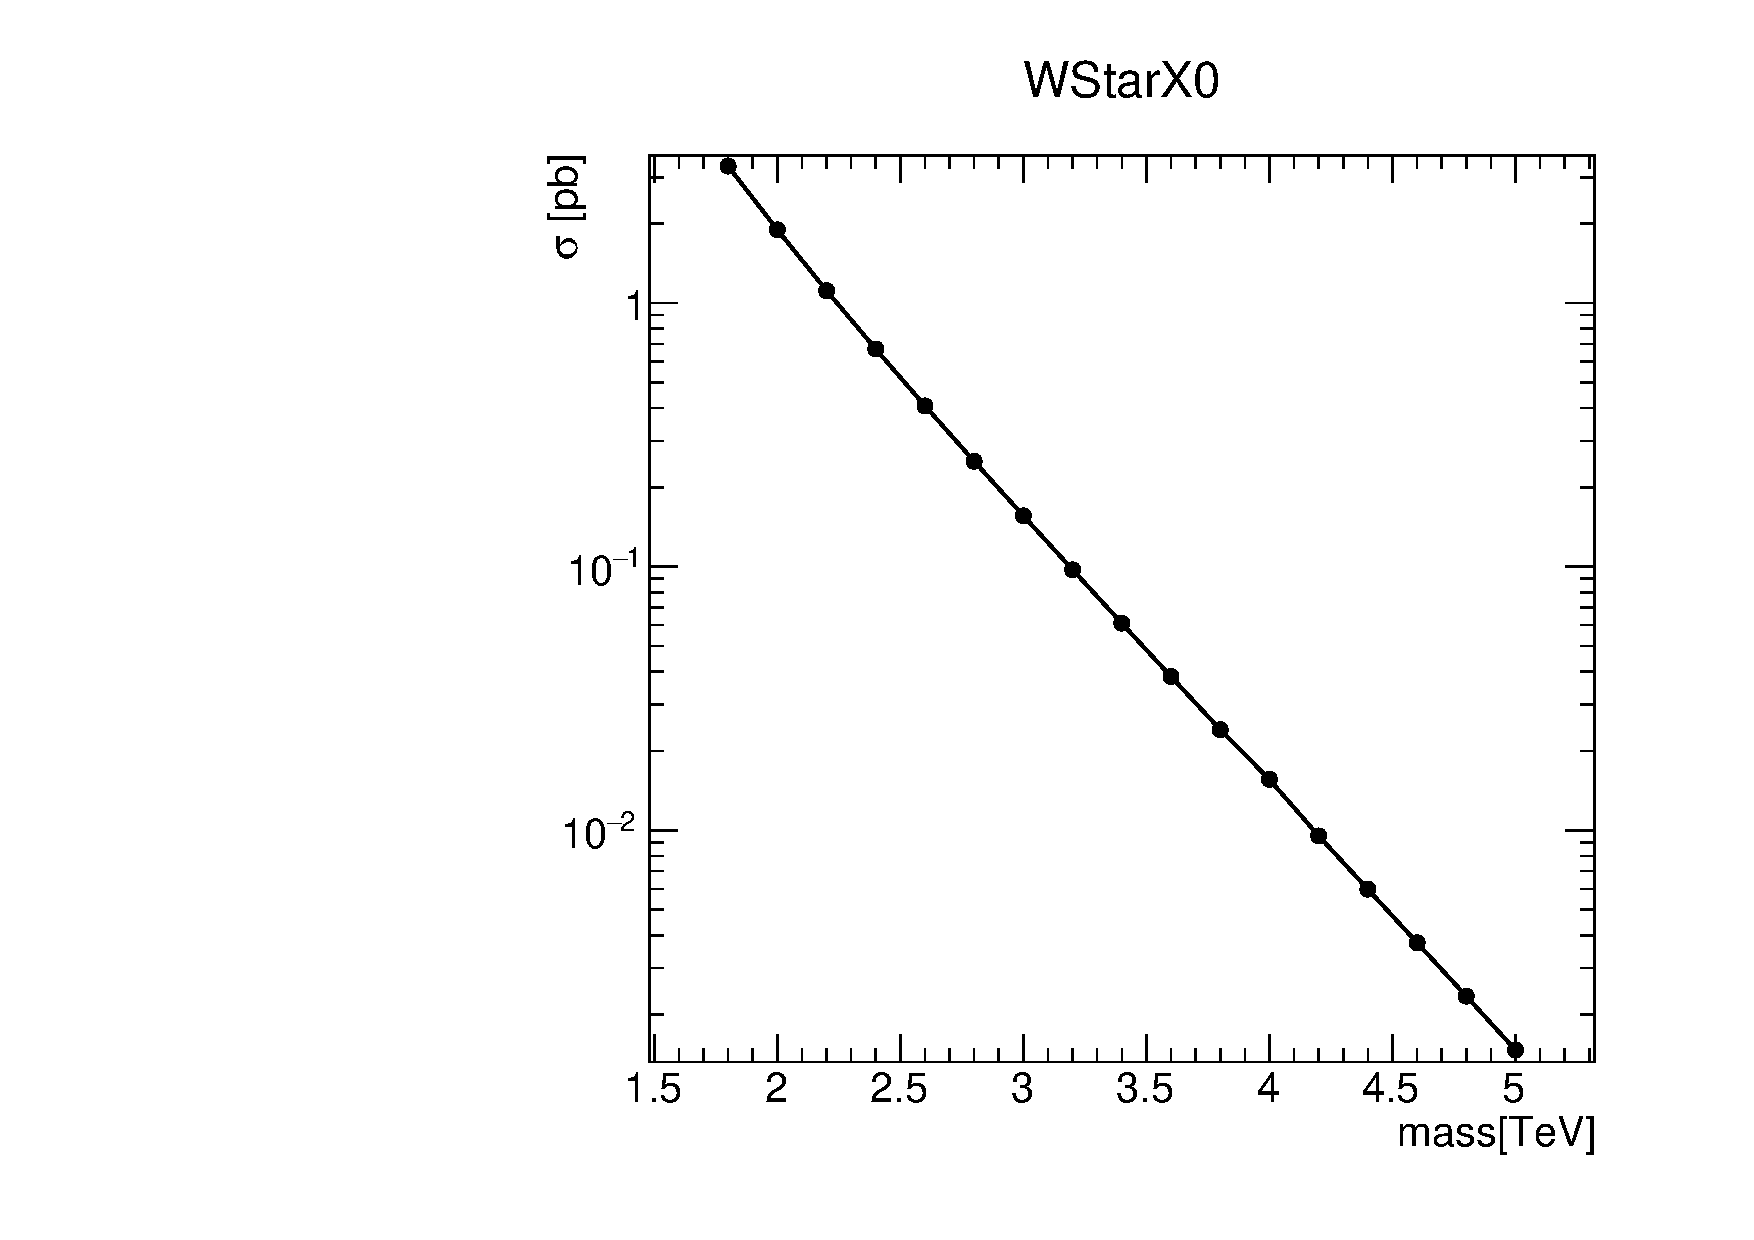
\includegraphics[width=0.48\textwidth]{figures/Wstar/CrossAcceptance/WstarX0_XS.pdf}}
  \subfigure[Acceptance]{\label{fig:Wstar_acc}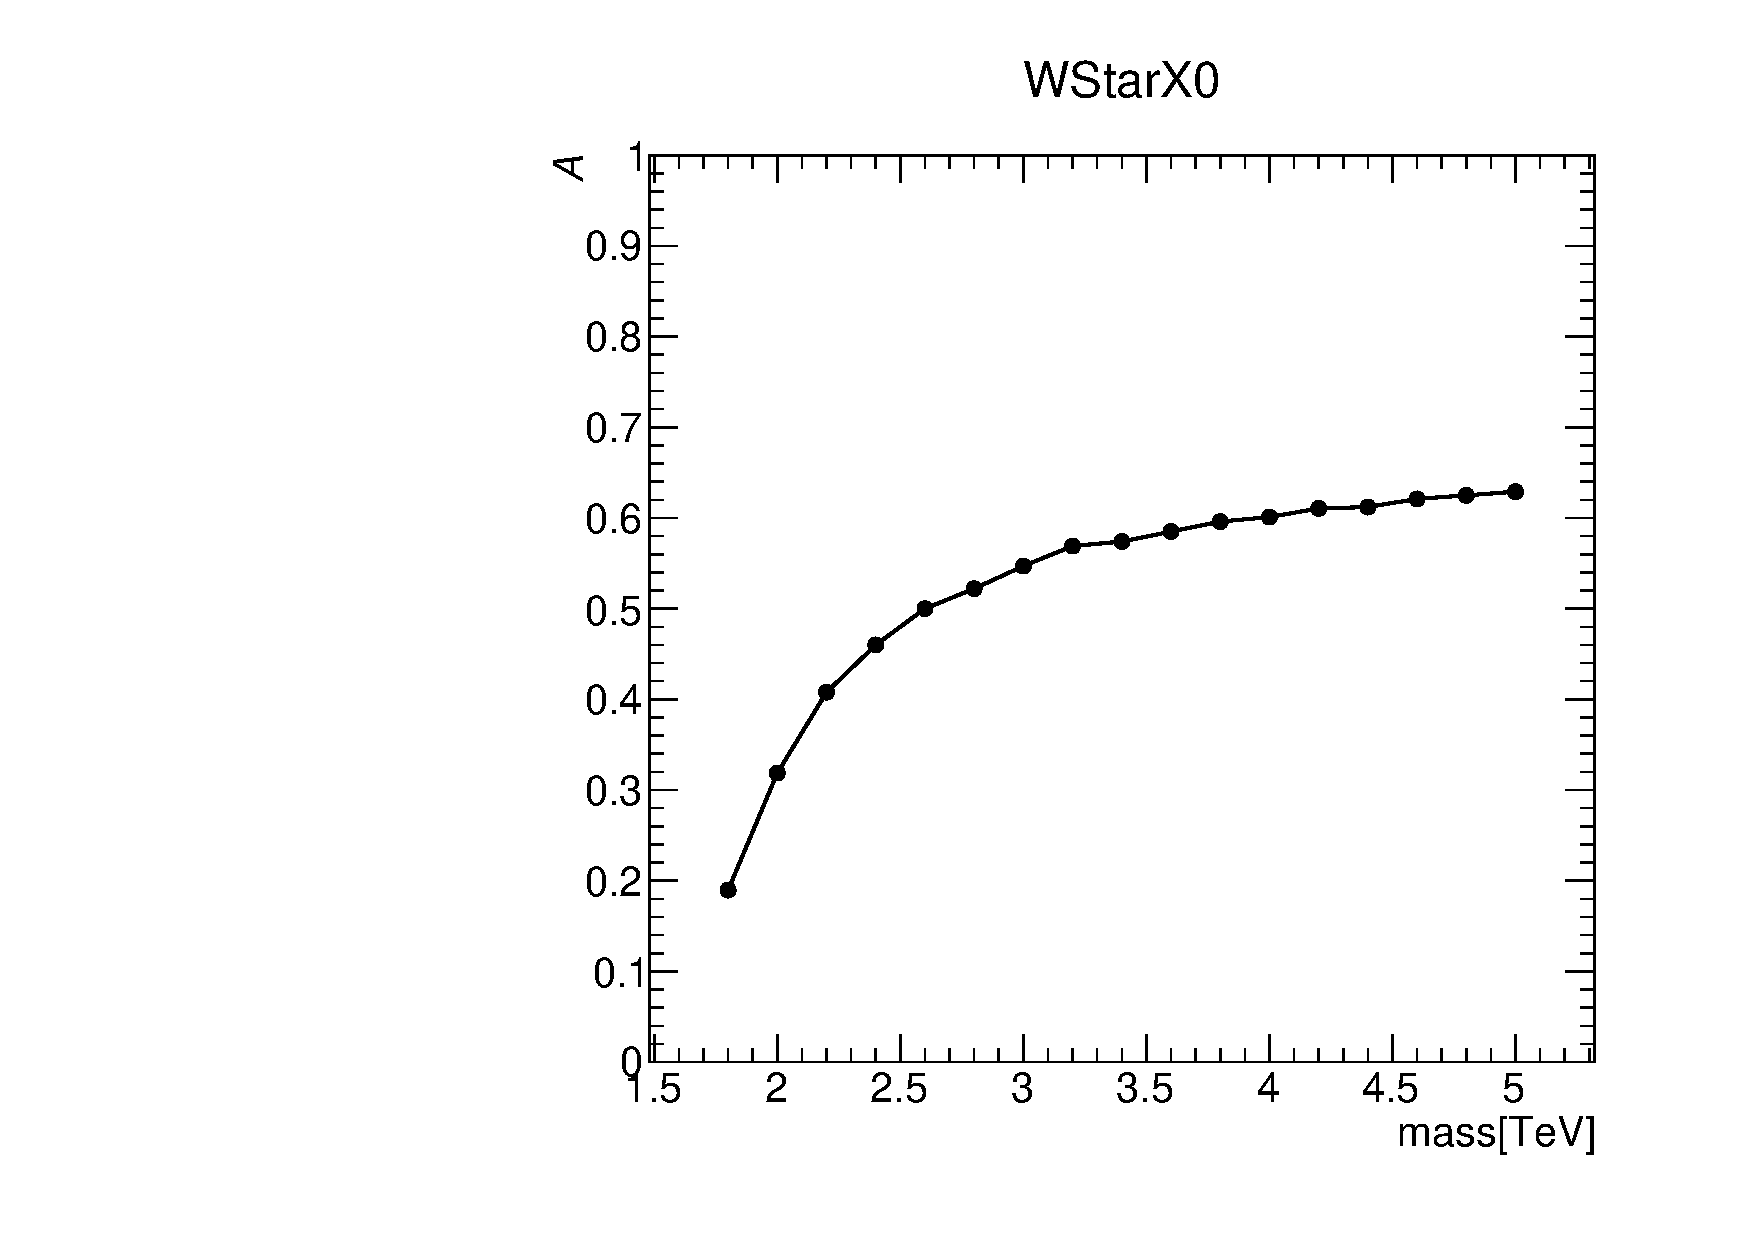
\includegraphics[width=0.48\textwidth]{figures/Wstar/CrossAcceptance/WstarX0_Acc.pdf}}
	\caption{(a) Cross section and (b) acceptance for the 
		\Wstar\ model for 13 TeV center-of-mass energies using the full resonance analysis selection (Section~\ref{sec:event_selection} except |y*|<1.2).
		%   The interpolation between points is a straight line therefore the 
		%   acceptance between m=1~\TeV~and m=2~\TeV~is not an accurate representation of
		%   what the acceptance of a m=1.5~\TeV~sample would be.  The interpolation
		%   is not used but drawn to help guide the eye.
        }
\end{figure}


%%%%%%%%%%%%%%%%%%%%%%%%%%%%%%%%%%%%%%%%%%%%%%%%%%%%%%%%%%%%%%%%%%%%%%%%%%%%%%%%
 \clearpage
 \subsubsection{Quantum black holes in the horizon quantum mechanics model}

The quadratically divergent corrections to the Higgs self-energy is a
well known problem of the Standard Model.
Supersymmetry offers a solution to this problem by fine-tuning the
cancellation. 
Alternatively, in low-scale string theory quadratic divergences are 
cutoff by the string mass scale, thus avoiding the fine-tuning problem.
In addition, superstring theory can act as a unifying framework between
TeV-scale Standard Model physics and Planck-scale quantum gravity.  

Superstring theory provides a braneworld description of the Standard
Model, which is localized on membranes extending in $p+3$ spatial
dimension, the so-called D-branes of dimension $p$: D$p$-branes.
D-branes can thus be used to connect string theory to
phenomenology~\cite{Antoniadis:2000ena,Cremades:2002qm,Antoniadis:2002qm}
Gauge bosons are due to strings attached to stacks of D-branes, and
chiral matter is due to strings stretching between intersecting D-branes.
The gauge interactions emerge as excitations of open strings with endpoints
attached on the D-branes, whereas gravitational interaction are described
by closed strings that can propagate in all nine spatial dimensions of
superstring theory.

We consider type-II string theory compactified on a six-dimensional
torus, which includes a D$p$-brane wrapped around $p-3$ dimensions of the
torus, with the remaining dimensions along our familiar (uncompactified)
three spatial dimensions.

The string mass-scale \Ms can be chosen hierarchically smaller than the
four-dimensional Planck scale at the expense of introducing $9-p$ large
transverse dimensions felt only by gravity, while keeping the string
coupling small~\cite{Cullen:2000ef}.
We are interested in the fundamental string scale in the TeV range.
The weakness of the effective four-dimensional gravity compared to gauge
interactions is then attributed to the large transverse space radii
compared to the string length; the so called AADD
model~\cite{ArkaniHamed:1998rs,Antoniadis:1998ig}. 

The string coupling must be small for the validity of the above D-brane
framework and of perturbation theory in the computation of scattering
amplitudes. 
If AADD is valid, string resonances will likely appear before gravity
signatures.
In this case, black hole production and other strong gravity effects
occur at energies above the string scale.
Thus, at least the lowest few Regge recurrences, are available for
examination, free from interference with some complex quantum
gravitational phenomena. 
The dominance of string resonances over Kaluza-Klein effects and winding
states is a generic feature of weakly coupled string
theory~\cite{Cullen:2000ef}. 
We do not considering the Kaluza-Klein states of the graviton in the
extra dimensions or the winding states.

In this framework, a whole tower of infinite string excitations will
open up at this low-mass threshold, and new particles of spin $J$ will
follow the well-known Regge trajectories of vibrating
strings.  
The string mass scale determines the centre of mass energy threshold 
for the production of Regge resonances in parton collisions, thus
corresponds to the onset of string effects at the LHC.

We consider dominant subprocesses in dijet production that are
independent of the details of compactification and are essentially
parameter free. 
Amplitudes, which include $2\to 2$ scattering processes involving four
gluons, or two gluons and two quarks, are independent of the details of
the compactification such as the configuration of branes, the geometry
of the extra dimensions, and whether SUSY is broken or
not~\cite{Lust:2008qc}. 
This model independence makes it possible to compute the string
corrections to QCD dijet processes.

The string resonances occur at masses $m_n = \sqrt{n} \Ms$, for $n = 1,
2, 3, \ldots$.
We only consider the first $(n=1)$ resonant pole.
The resonance will consist of a combination of the Regge excitations of
the quark, the gluon, and the colour singlet living on the QCD stack of
branes. 
The string-resonance widths have been calculated in
Ref~\cite{Anchordoqui:2008hi}. 

First phenomenological studies were done in
Ref~\cite{Anchordoqui:2007da,Anchordoqui:2009mm,Kitazawa:2010gh,Anchordoqui:2014wha}. 
Searches for string resonances have been performed in previous dijet
mass spectra.
ATLAS~\cite{ATLAS:2012pu} searched in 4.8~fb$^{-1}$ of data at $\sqrt{s}
= 7$~TeV.
A lower limit of $\Ms < 3.61$~TeV at a 95\% CL was set.
The MC signal samples were provided by a non-ATLAS member Noriaki
Kitazawa who used CalcHEP.
CMS~\cite{Chatrchyan:2011ns,CMS:2012yf} performed two searches in dijets
at $\sqrt{s} = 7$~TeV.
Lower limits of $\Ms < 4.00$~TeV and $\Ms < 4.31$~TeV were set at the
95\% CL using datasets of 1.0~fb$^{-1}$ and 5.0~fb$^{-1}$, respectively. 
It is not totally clear how this limit was set but the excited
quark MC sample was probably used for the signal event generation. 
A non-CMS member Can Kilic did the string resonance cross section
calculation. 
CMS~\cite{Khachatryan:2015sja} performed the only search at $\sqrt{s} =
8$~TeV using 19.7~fb$^{-1}$ of data, to obtain a lower limit of $\Ms <
5.0$~TeV at the 95\% CL.
The paper does not explanation of how this limit was calculated.
CMS~\cite{Khachatryan:2015dcf,Sirunyan:2018xlo} performed two searches
in dijets at $\sqrt{s} = 13$~TeV. 
Lower limits of $\Ms < 7.0$~TeV and $\Ms < 7.7$~TeV were set at the
95\% CL using datasets of 2.4~fb$^{-1}$ and 36~fb$^{-1}$, respectively. 
Again, no explanation of the signal samples are given and only the $gq$
state is considered.
Both experiments have performed searches for string balls in different
decay modes at $\sqrt{s} = 7, 8$, and 13~TeV, but we argue that the
model~\cite{Gingrich:2008di} used does not constrain string resonances,
or visa versa. 
%%%%%%%%%%%%%%%%%%%%%%%%%%%%%%%%%%%%%%%%%%%%%%%%%%%%%%%%%%%%%%%%%%%%%%%%%%%%%%%%

%%%%%%%%%%%%%%%%%%%%%%%%%%%%%%%%%%%%%%%%%%%%%%%%%%%%%%%%%%%%%%%%%%%%%%%%%%%%%%%%
Five string-resonance samples with string scales \Ms from 7.0~TeV to
9.0~TeV, in steps of 0.5~TeV are generated.
The minimum mass $M_\mathrm{min}$ used in the generator and the
resulting cross section of the samples are shown in Table~\ref{tab1}. 

\begin{table}[htb]
\begin{center}
\begin{tabular}{ccc}\hline\\[-2ex]
\Ms & $M_\mathrm{min}$ & Cross section\\
{[TeV]} & {[TeV]} & {[fb]}\\ \\[-2ex]
\hline\\[-2ex]
7.0 & 6.06 & $7.09\times 10^{+0}$\\
7.5 & 6.60 & $1.86\times 10^{+0}$\\
8.0 & 7.14 & $4.56\times 10^{-1}$\\
8.5 & 7.60 & $1.00\times 10^{-1}$\\
9.0 & 8.05 & $1.99\times 10^{-2}$\\
\\[-2ex]\hline
\end{tabular}
\end{center}
\caption{Monte Carlo string-resonance samples with string scale \Ms,
minimum mass $M_\mathrm{min}$, and cross section.} 
\label{tab1}
\end{table}

The string resonances have long Breit-Wigner tails and the lower-mass
tail can be significantly enhanced by the PDFs at low-$x$ (low mass).
Since we are interested in a narrow-resonance structure in the dijet
mass distribution, we truncate the low-mass tail.
For the $7.0 \leq \Ms \leq 8.0$~TeV samples, we truncate at the minimum in
the differential cross section on the lower-mass side of the \Ms peak,
which results in including slightly more than 95\% of the area under the
curve. 
For the $8.5 \leq \Ms \leq 9.0$~TeV samples, we truncate at a lower-mass
value that covers 95\% of the area under the Breit-Wigner curve.

Five possible $2\to 2$ subprocesses that can give rise to string
resonances are simulated.
The cross section for each subprocess is a function of \Ms, and thus the
relative contribution of each subprocess to the total cross section varies
with \Ms, as shown in Table~\ref{tab2}.
The dominate subprocess at the \Ms values we consider is $gq\to gq$ which
contributes about 81-87\% of the total cross section.
Previous ATLAS and CMS searches only included the dominate subprocess.
The $qq\to qq$, $\bar{q}\bar{q}\to \bar{q}\bar{q}$, and $q\bar{q}\to
q\bar{q}$ subprocesses are model dependent, and not
considered here.

\begin{table}[htb]
\begin{center}
\begin{tabular}{crrrrr}\hline\\[-2ex]
Subprocess             & \multicolumn{5}{c}{\Ms\ {[TeV]}}\\
& \multicolumn{1}{c}{7.0} & \multicolumn{1}{c}{7.5} &
\multicolumn{1}{c}{8.0} & \multicolumn{1}{c}{8.5} &
\multicolumn{1}{c}{9.0}\\ \\[-2ex]
\hline\\[-2ex]
$gg\to gg$             & 11.36\% &  9.52\% &  8.17\% &  7.23\% &  5.07\%\\
$gg\to q\bar{q}$       &  0.29\% &  0.28\% &  0.22\% &  0.19\% &  0.17\%\\
$gq\to gq$             & 81.36\% & 83.12\% & 84.58\% & 85.54\% & 87.59\%\\
$g\bar{q}\to g\bar{q}$ &  0.68\% &  0.58\% &  0.52\% &  0.51\% &  0.49\%\\
$q\bar{q}\to gg$       &  6.31\% &  6.50\% &  6.51\% &  6.53\% &  6.67\%\\
\\[-2ex] \hline
\end{tabular}
\end{center}
\caption{String-resonance subprocesses and their relative contribution
to the total cross section for different string scales \Ms.
The statistics are based on samples of 66000 events.}
\label{tab2}
\end{table}

For the string-resonance samples, the MC event
generator \str~1.00~\cite{Vakilipourtakalou:2018pfo} is used.
It is interfaced to \pythia~8.240~\cite{Sjostrand:2014zea} for modelling
of the parton shower, hadronization, and underlying event, with
parameters from the A14 tune~\cite{ATL-PHYS-PUB-2014-021}.
The leading-order CTEQ6L1~\cite{Pumplin:2002vw} PDF set is used for the
parton shower and the hard-scattering process.
The EvtGen~1.6.0 program~\cite{Lange:2001uf} is used to decay bottom
and charm hadrons. 

The effect of multiple interactions in the same and neighbouring bunch
crossings (pile-up) is modelled by overlaying simulated inelastic $pp$
events generated with \pythia~8.186~\cite{Sjostrand:2014zea}
using NNPDF2.3LO set of PDFs~\cite{Ball:2012cx} and the A3
tune~\cite{ATL-PHYS-PUB-2016-017} over the original hard-scattering event. 
%%%%%%%%%%%%%%%%%%%%%%%%%%%%%%%%%%%%%%%%%%%%%%%%%%%%%%%%%%%%%%%%%%%%%%%%%%%%%%%%

\clearpage
\subsubsection{Signal shapes in the various models}

The shape of the signal peak for each mass point and each signal model, after the resonance selection cuts, are shown in Figure~\ref{fig:showallshapes}. Each template is normalised to 1, and therefore differences in peak amplitude are indicative of a broadening or narrowing of the signal rather than of a change in cross section.
\begin{figure}[!htb]
\centering
\subfigure[q* model]{\label{fig:resonance_templates_2500}
               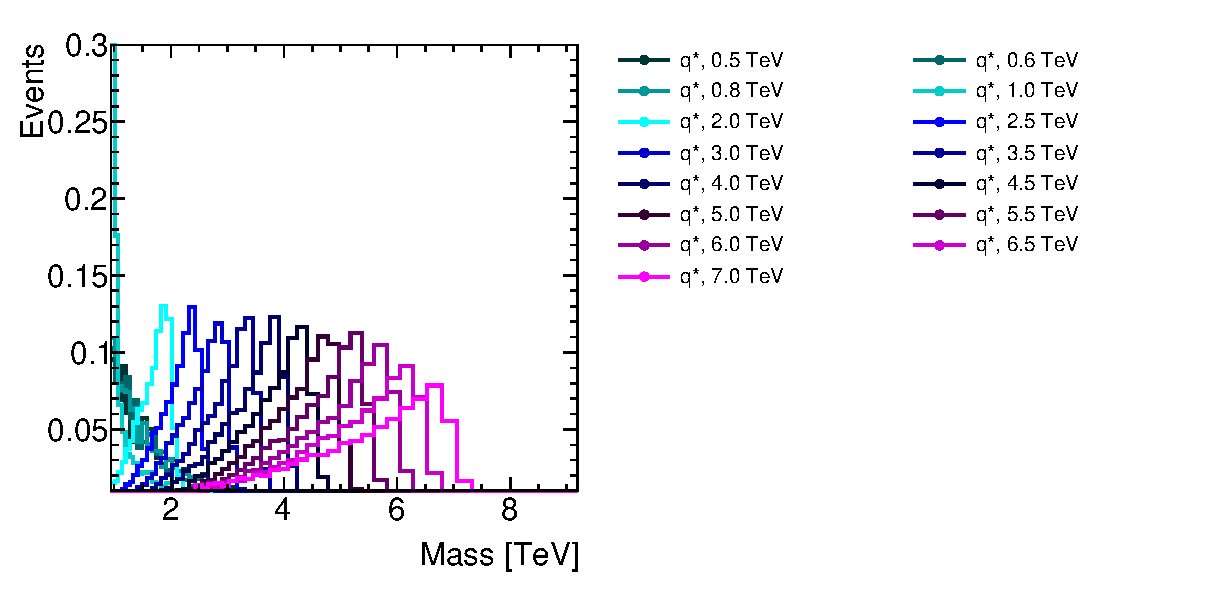
\includegraphics[height=0.25\textwidth]{figures/benchmark_signals/overlaidQStar_mjj_linear.eps}}
\subfigure[\BlackMax\ model]{\label{fig:resonance_templates_4500}
               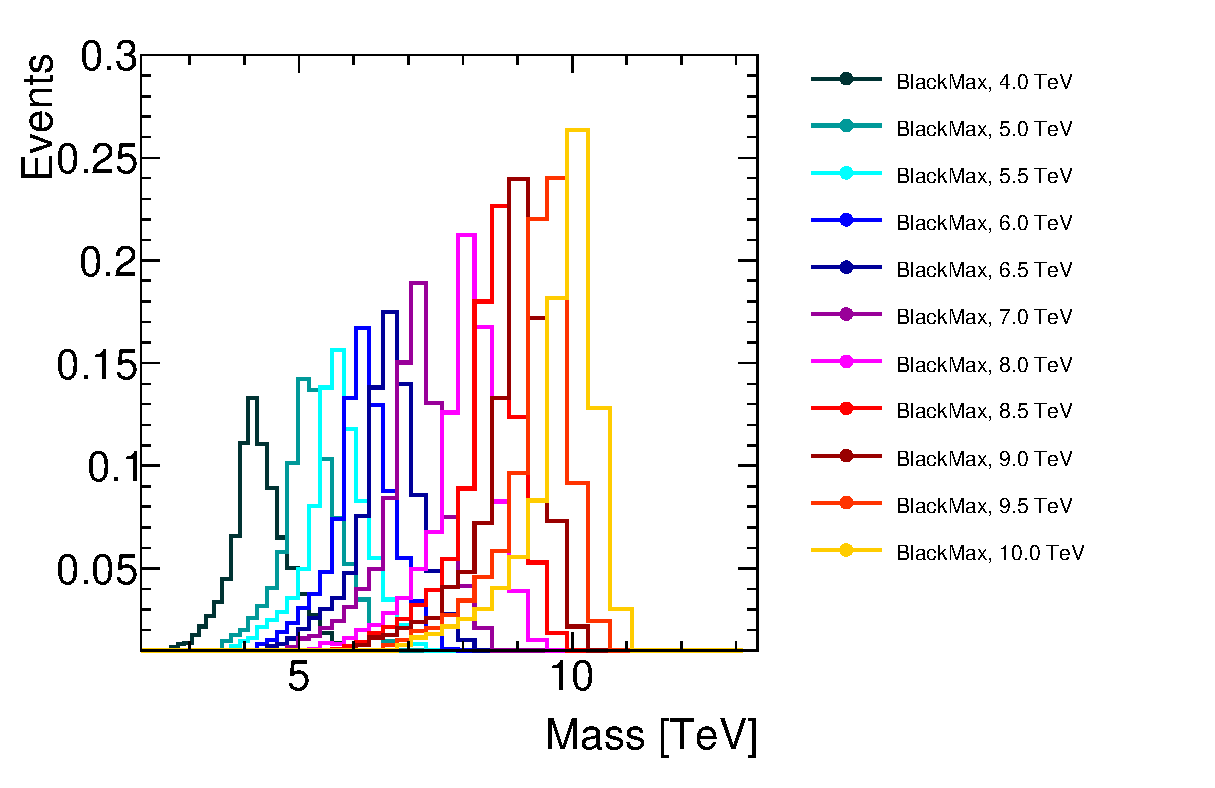
\includegraphics[height=0.25\textwidth]{figures/benchmark_signals/overlaidBlackMax_mjj_linear.eps}}
\subfigure[\Wprime\ model]{\label{fig:resonance_tr_templates_2500}
               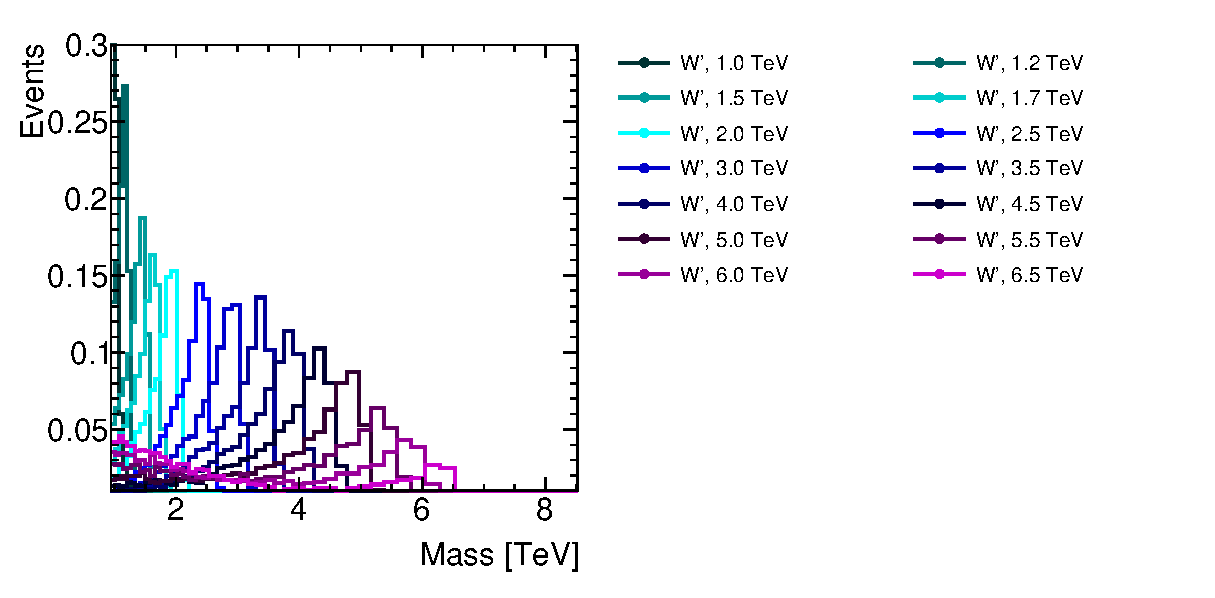
\includegraphics[height=0.25\textwidth]{figures/benchmark_signals/overlaidWPrime_mjj_linear.eps}}
\subfigure[\Wstar\ model]{\label{fig:showallshapes}
               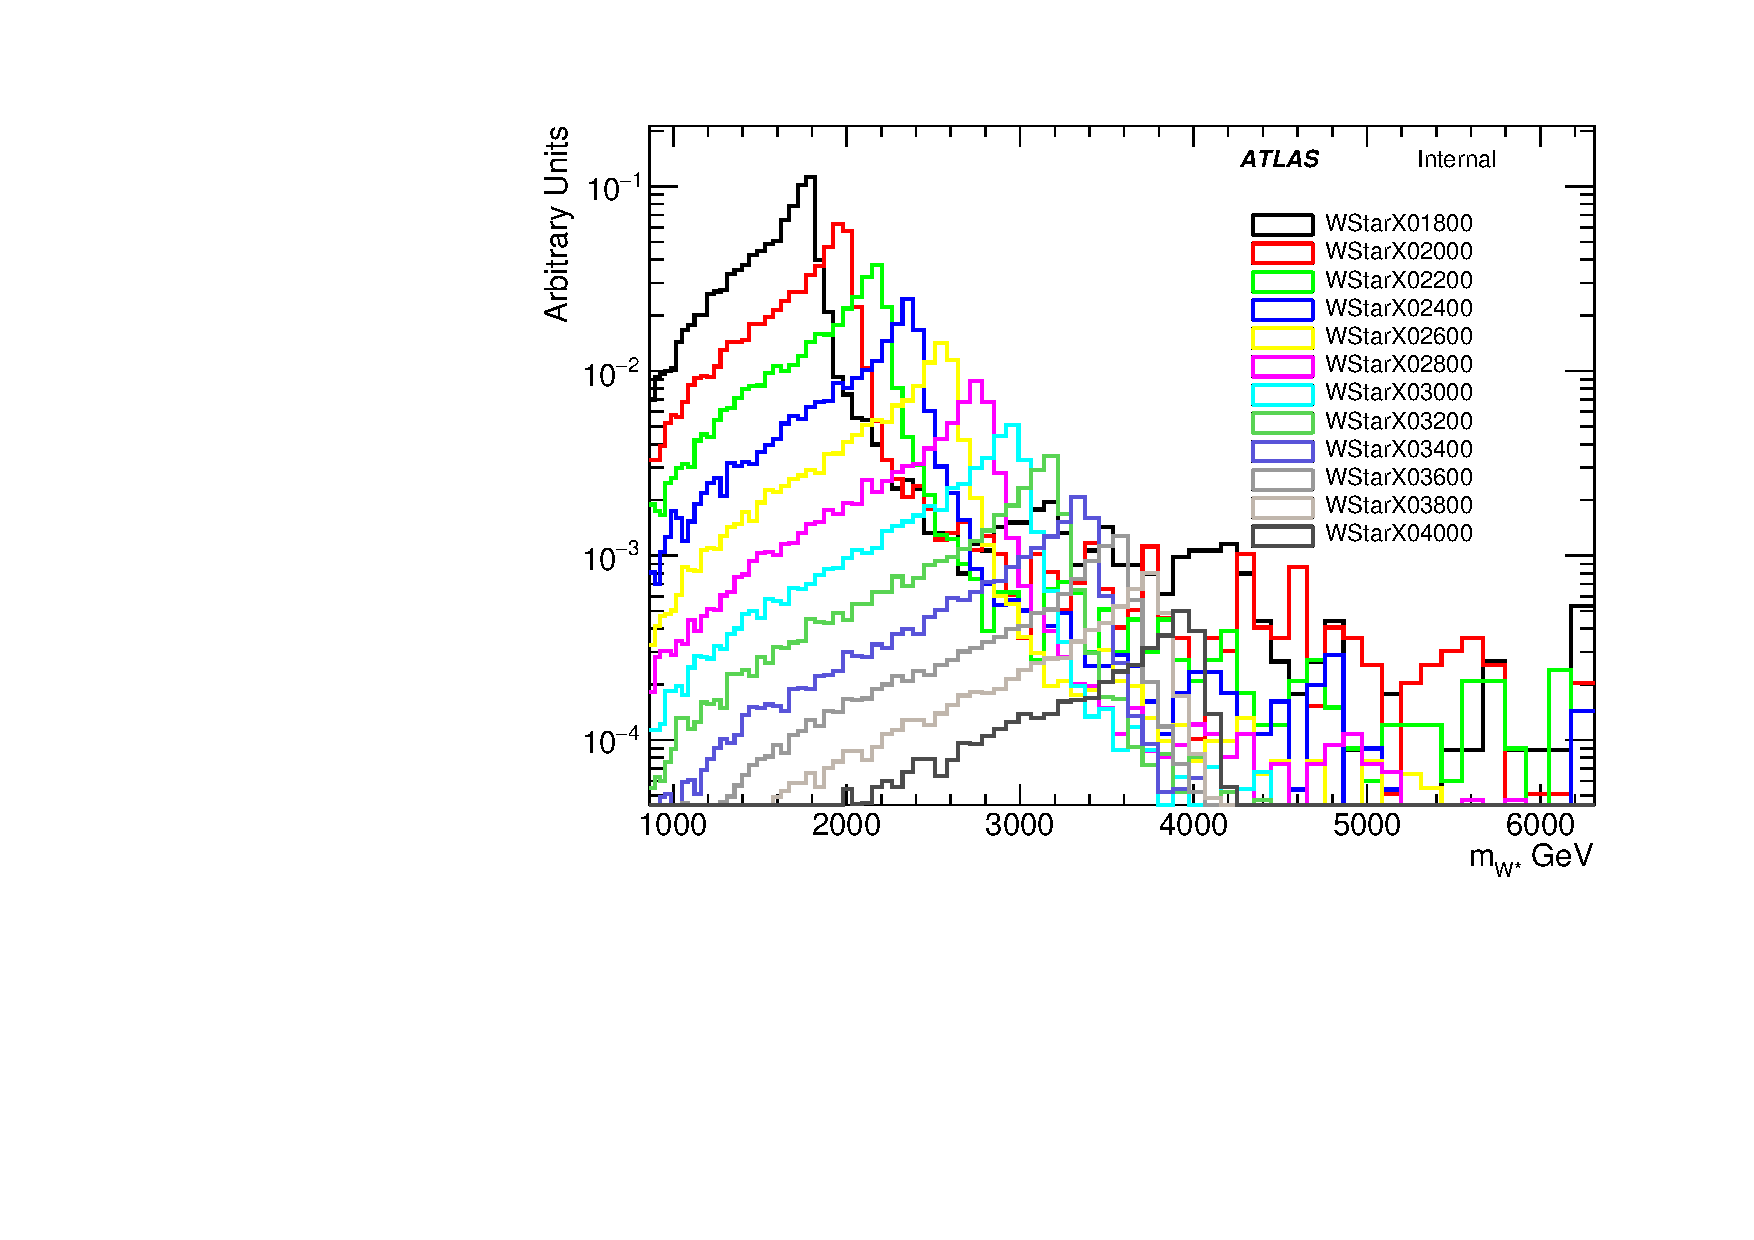
\includegraphics[height=0.25\textwidth]{figures/Wstar/CrossAcceptance/MassesDist.pdf}}
%\subfigure[4.5 TeV, truncated]{\label{fig:resonance_tr_templates_4500}
 %              \includegraphics[width=0.45\textwidth]{old_figures_2015/search_results/Resonance/Gaus_Comp/M4500_tr_comp.pdf}}
\caption{Normalized \mjj\ templates at every mass point considered in the limit setting phasse for each of the resonant benchmark models. }

\end{figure}

The benchmark signals used vary in their underlying physics motivation, but also in the resulting shape of the signal \mjj\ distribution. 
This is demonstrated most clearly in Figure~\ref{fig:resonance_templates_shapes}, which shows overlaid reconstructed \mjj\ distributions for a selection of benchmark signals at the same mass point.
The low-mass tail of \Wprime\ starts to become pronounced at higher masses, and the \qstar\ signal is also broadened. 
In contrast to the previous two, \BlackMax\ signals peak at masses slightly higher than the generated mass. 
The detailed differences between the signal shapes become apparent in Figures~\ref{fig:resonance_tr_templates_4000} and \subref{fig:resonance_tr_templates_6500}, 
which show the signal templates truncated at $\pm 20 \%$ of the generated mass. 
This is the truncation recommended for recasting of the generic Gaussian observed limits set by this analysis into signals with peaked but non-Gaussian \mjj\ distributions. 
The truncated distributions show that the \qstar\ signal distributions are shifted the most to lower \mjj\ of all signals, for both lower and higher masses. 
% 
% 
\begin{figure}[!htb]
\centering
\subfigure[4.0 TeV]{\label{fig:resonance_templates_4000}
               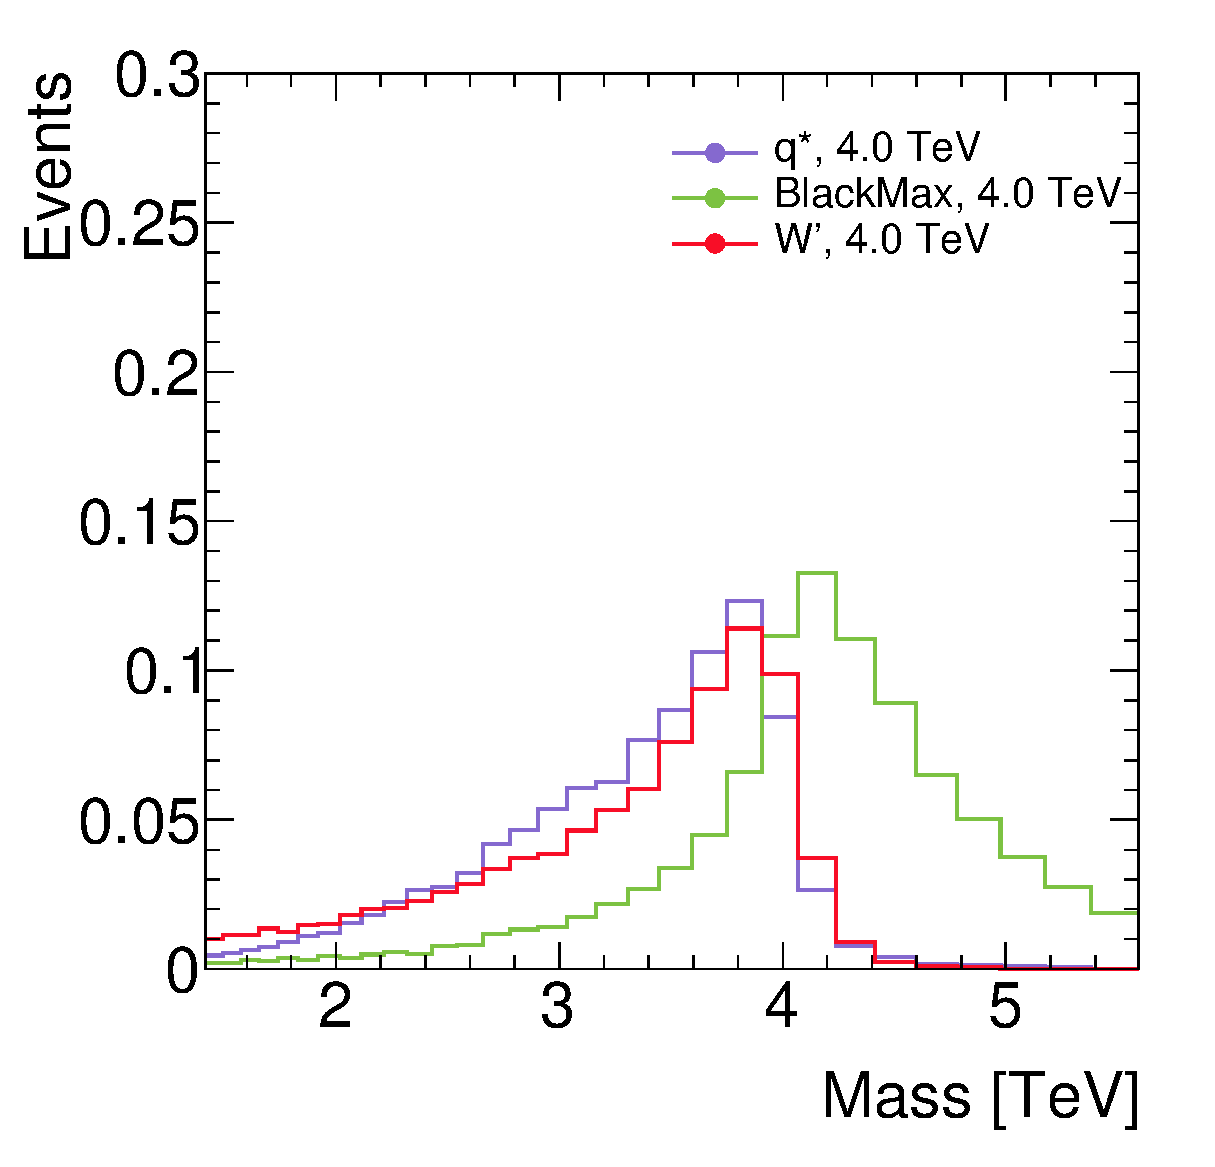
\includegraphics[width=0.45\textwidth]{figures/benchmark_signals/overlaidSignals_m4000_linear.eps}}
\subfigure[6.5 TeV]{\label{fig:resonance_templates_6500}
               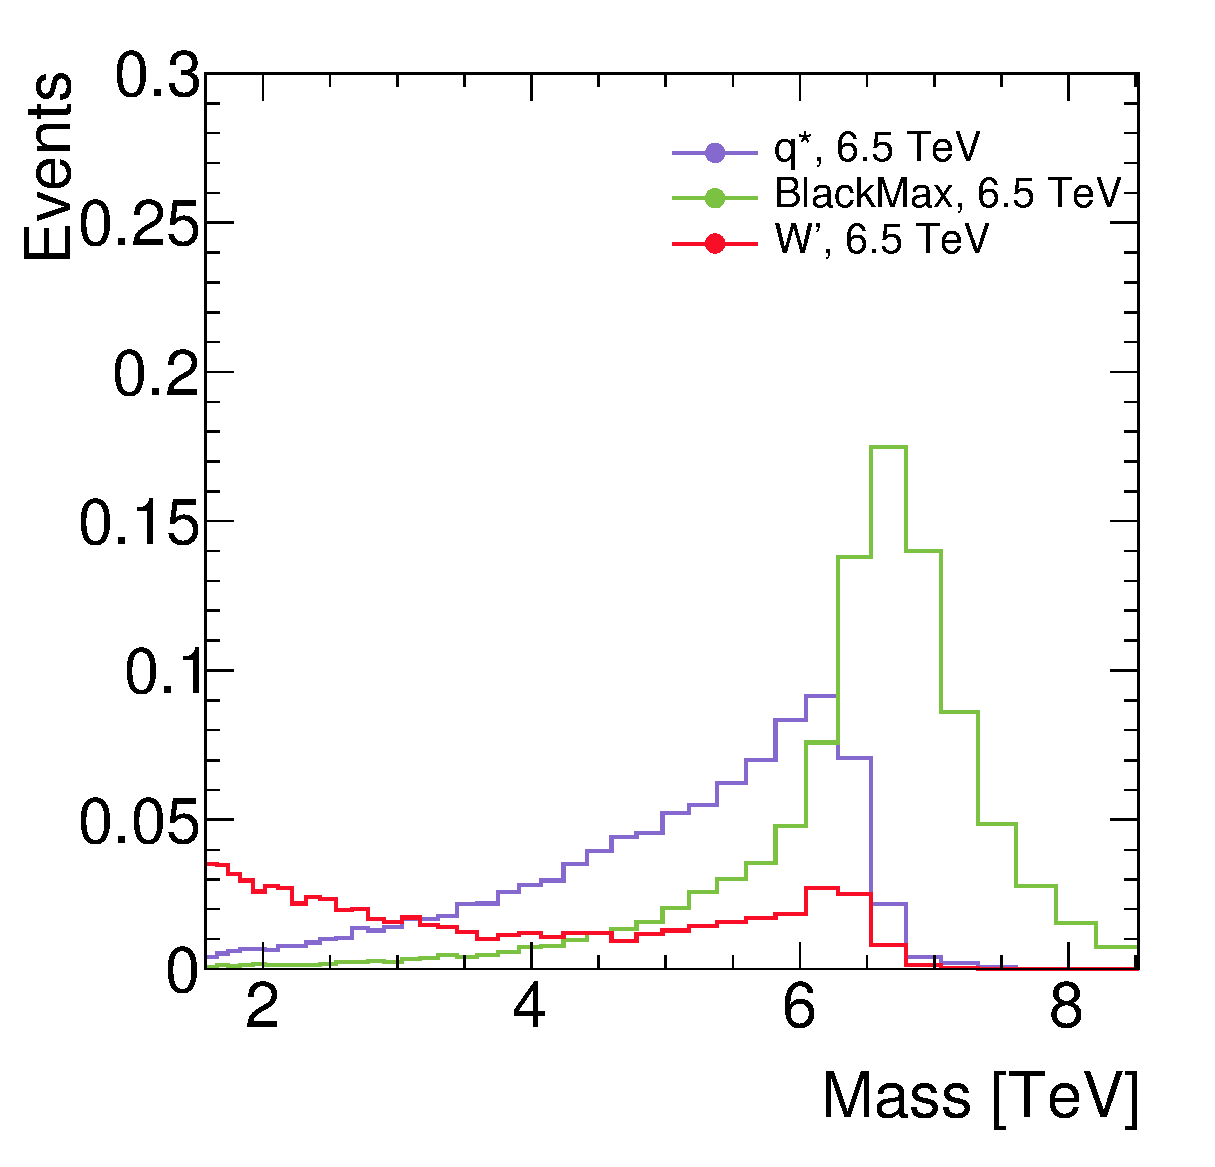
\includegraphics[width=0.45\textwidth]{figures/benchmark_signals/overlaidSignals_m6500_linear.eps}}
\subfigure[4.0 TeV, truncated]{\label{fig:resonance_tr_templates_4000}
               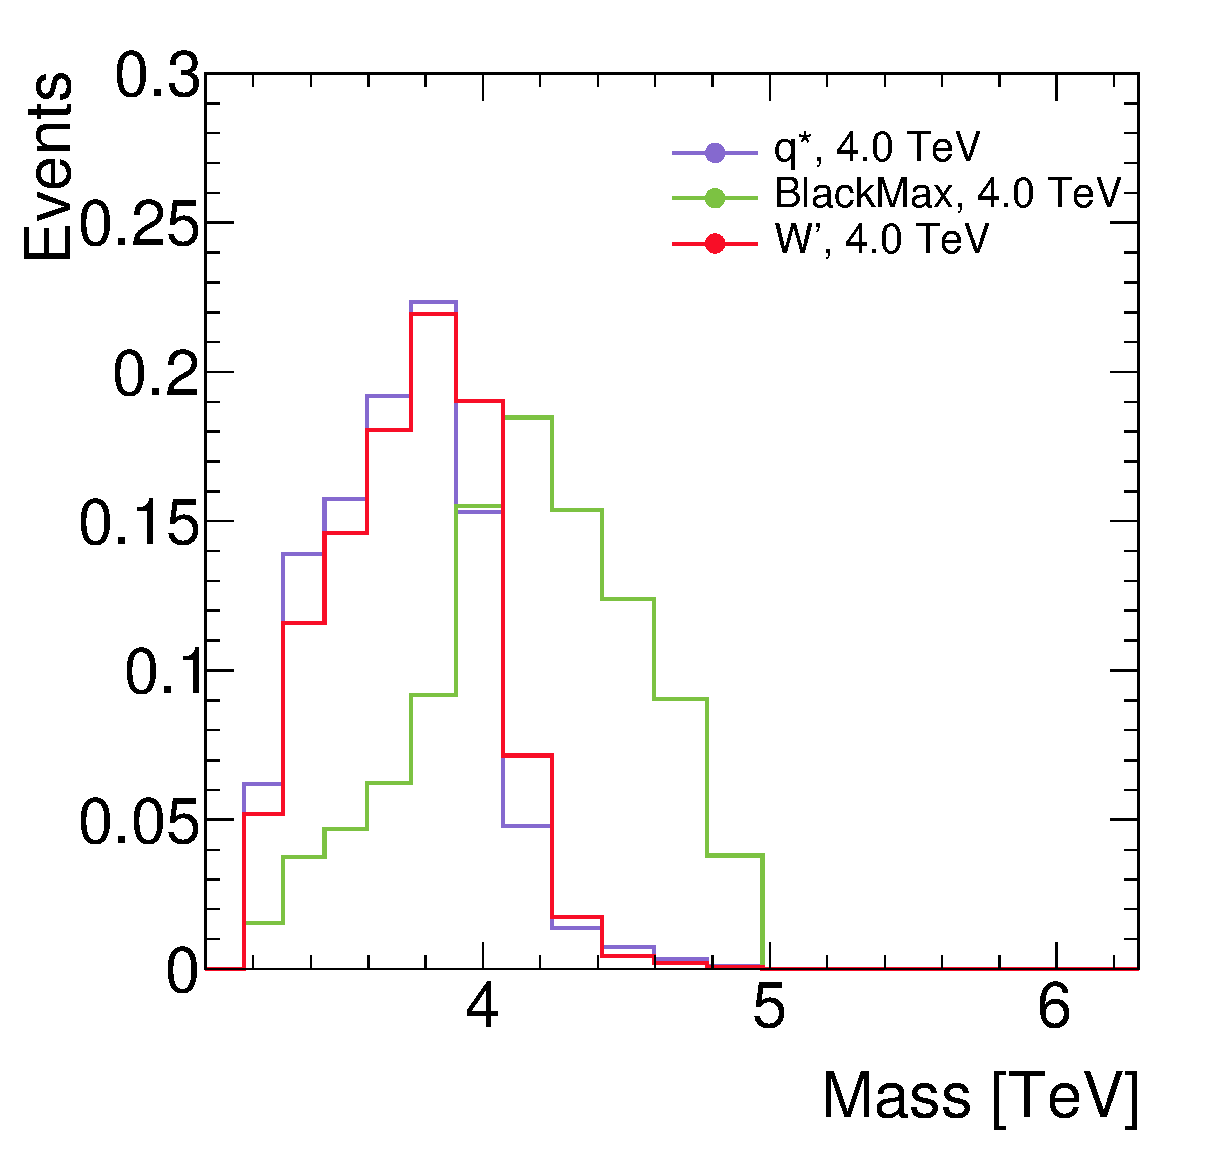
\includegraphics[width=0.45\textwidth]{figures/benchmark_signals/overlaidSignals_m4000_trunc.eps}}
\subfigure[6.5 TeV, truncated]{\label{fig:resonance_tr_templates_6500}
               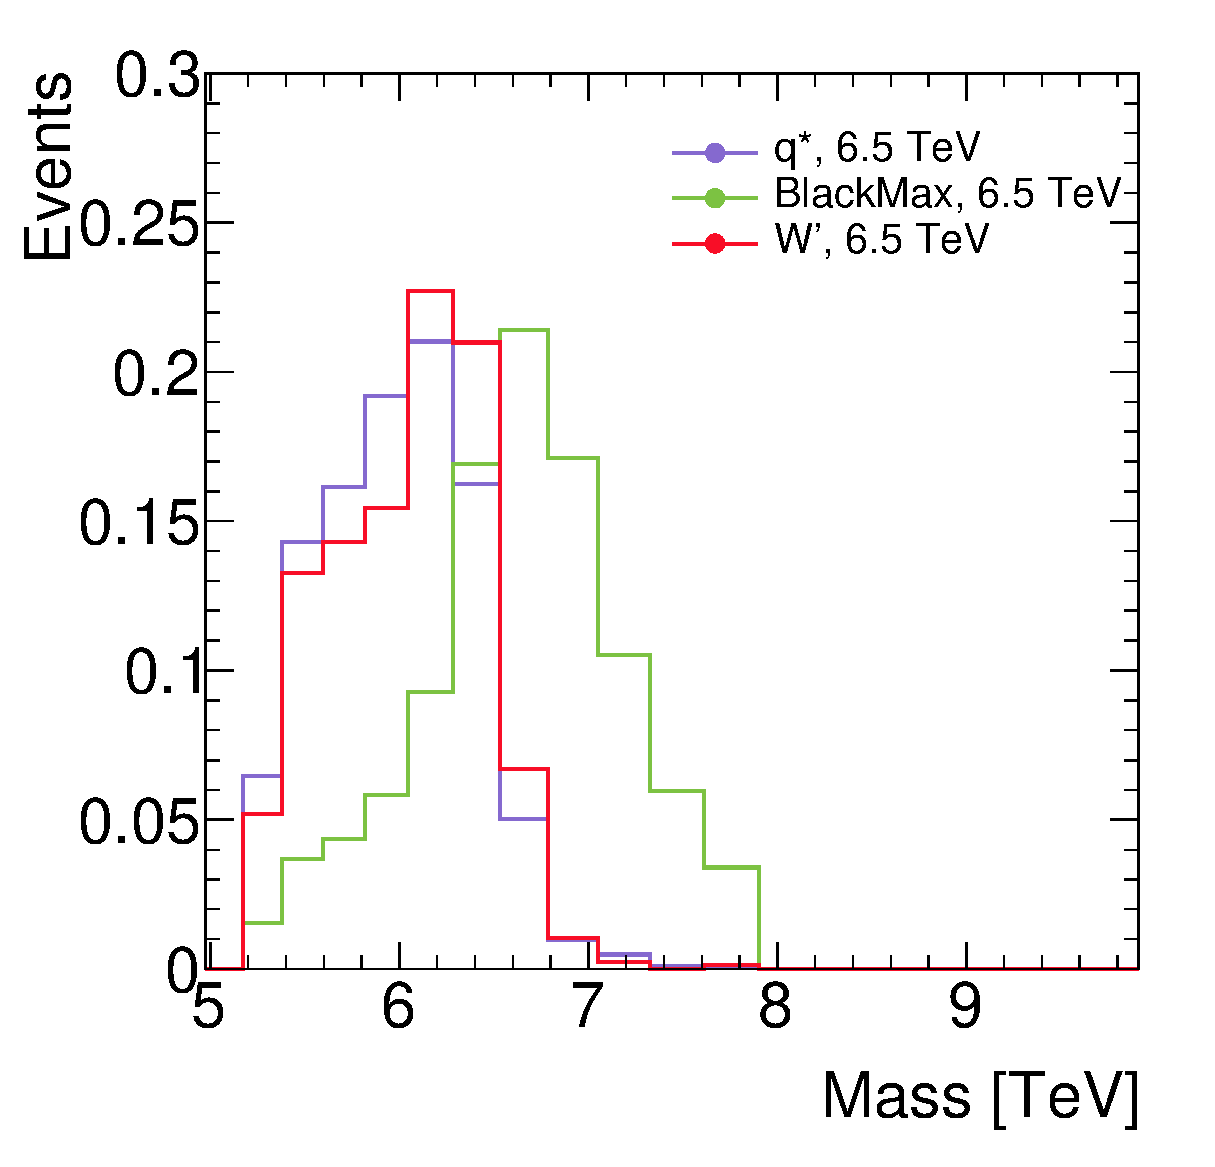
\includegraphics[width=0.45\textwidth]{figures/benchmark_signals/overlaidSignals_m6500_trunc.eps}}

\caption{Normalized \mjj\ templates at 4.0 TeV \subref{fig:resonance_templates_4000},\subref{fig:resonance_tr_templates_4000} and 6.5 TeV \subref{fig:resonance_templates_6500},\subref{fig:resonance_tr_templates_6500}, before (above) and after (below) the truncation procedure, for various resonant benchmark models. The signals are re-normalised after truncation for ease of comparison of the shapes.}
\label{fig:resonance_templates_shapes}
\end{figure}


\clearpage
%%%%%%%%%%%%%%%%%%%%%%%%%%%%%%%%%%%%%%%%%%%%%%%%%%%%%%%%%%%%%%%%%%%%
\subsubsection{Signal Morphing}
\label{sec:SwiftMorphing}
%%%%%%%%%%%%%%%%%%%%%%%%%%%%%%%%%%%%%%%%%%%%%%%%%%%%%%%%%%%%%%%%%%%%


Smooth signal mass distributions are obtained  from morphing the signal shapes from MC. The MC signals are fit to a Gaussian + reverse Landau function, a parameterization that has one normalization and five shape parameters. The parameters are interpolated as a function of mass using cubic splines. This allows the use of signal shapes at any mass. Figure~\ref{fig:morphing} shows some examples of fits to MC signal shapes as well as several interpolated signal shapes.  

\begin{figure}[!htb]
	\centering
	\subfigure[q* signals]{ 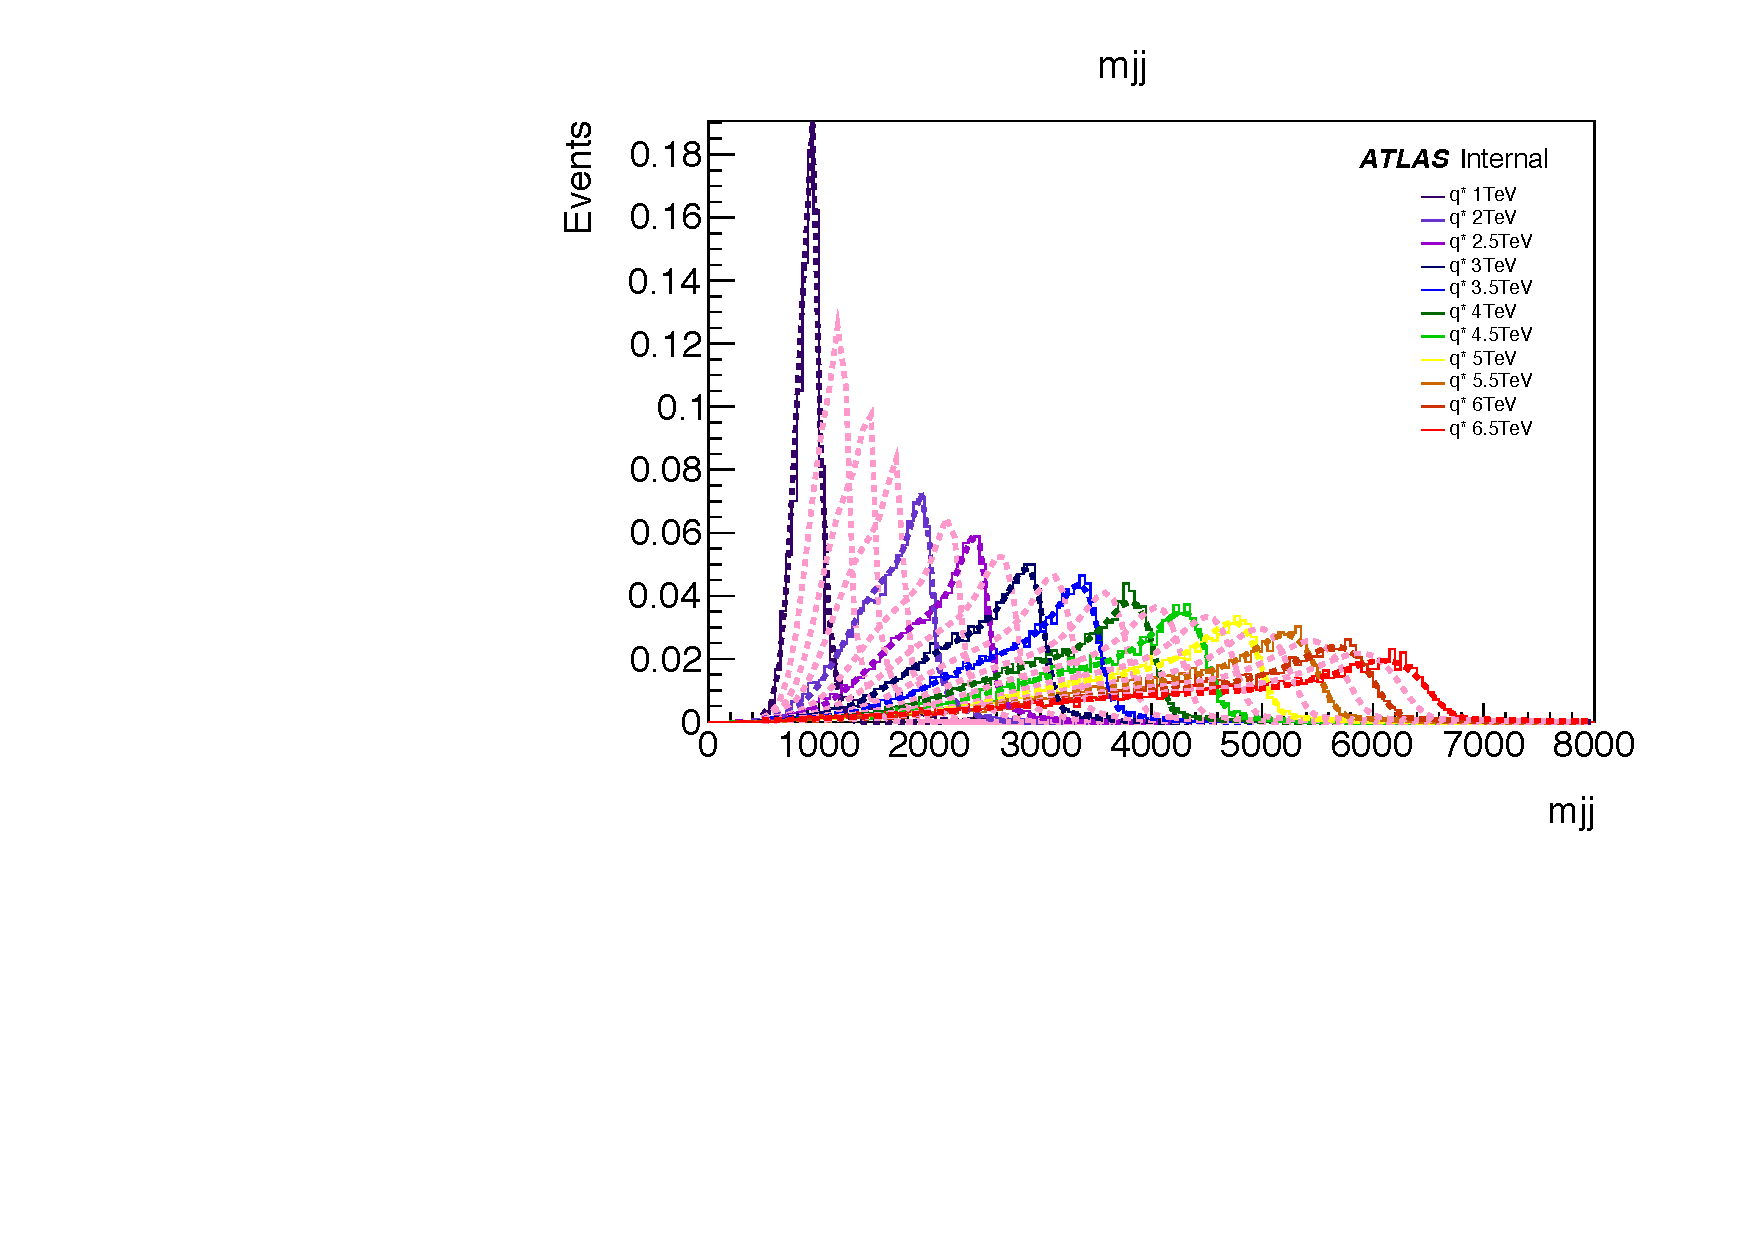
\includegraphics[width=0.48\textwidth]{figures/SWiFt/interpolate_qStar.pdf} }
	\subfigure[Reclustered W' signals]{ 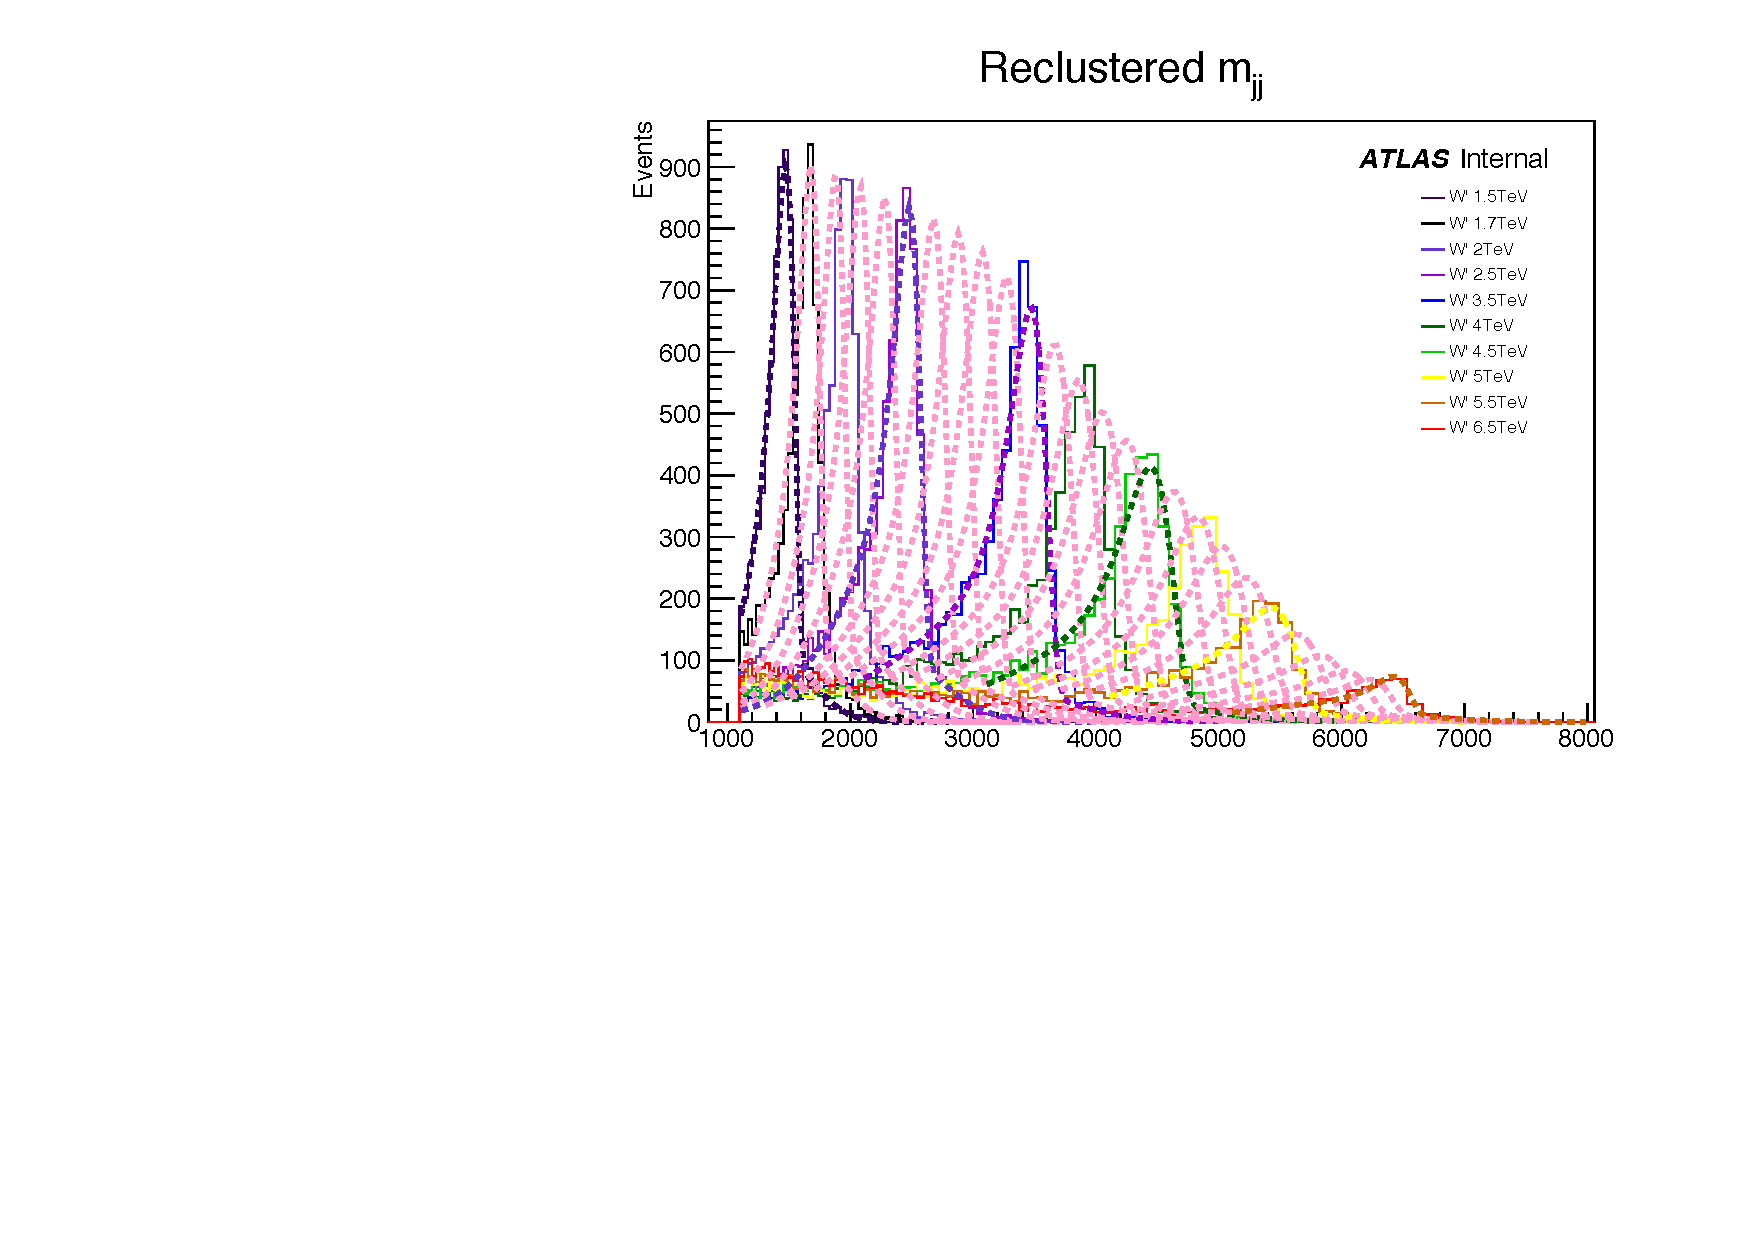
\includegraphics[width=0.48\textwidth]{figures/SWiFt/interpolate_WPrimeRe.pdf} }
	\subfigure[Z' 0.2 SM coupling signals]{ 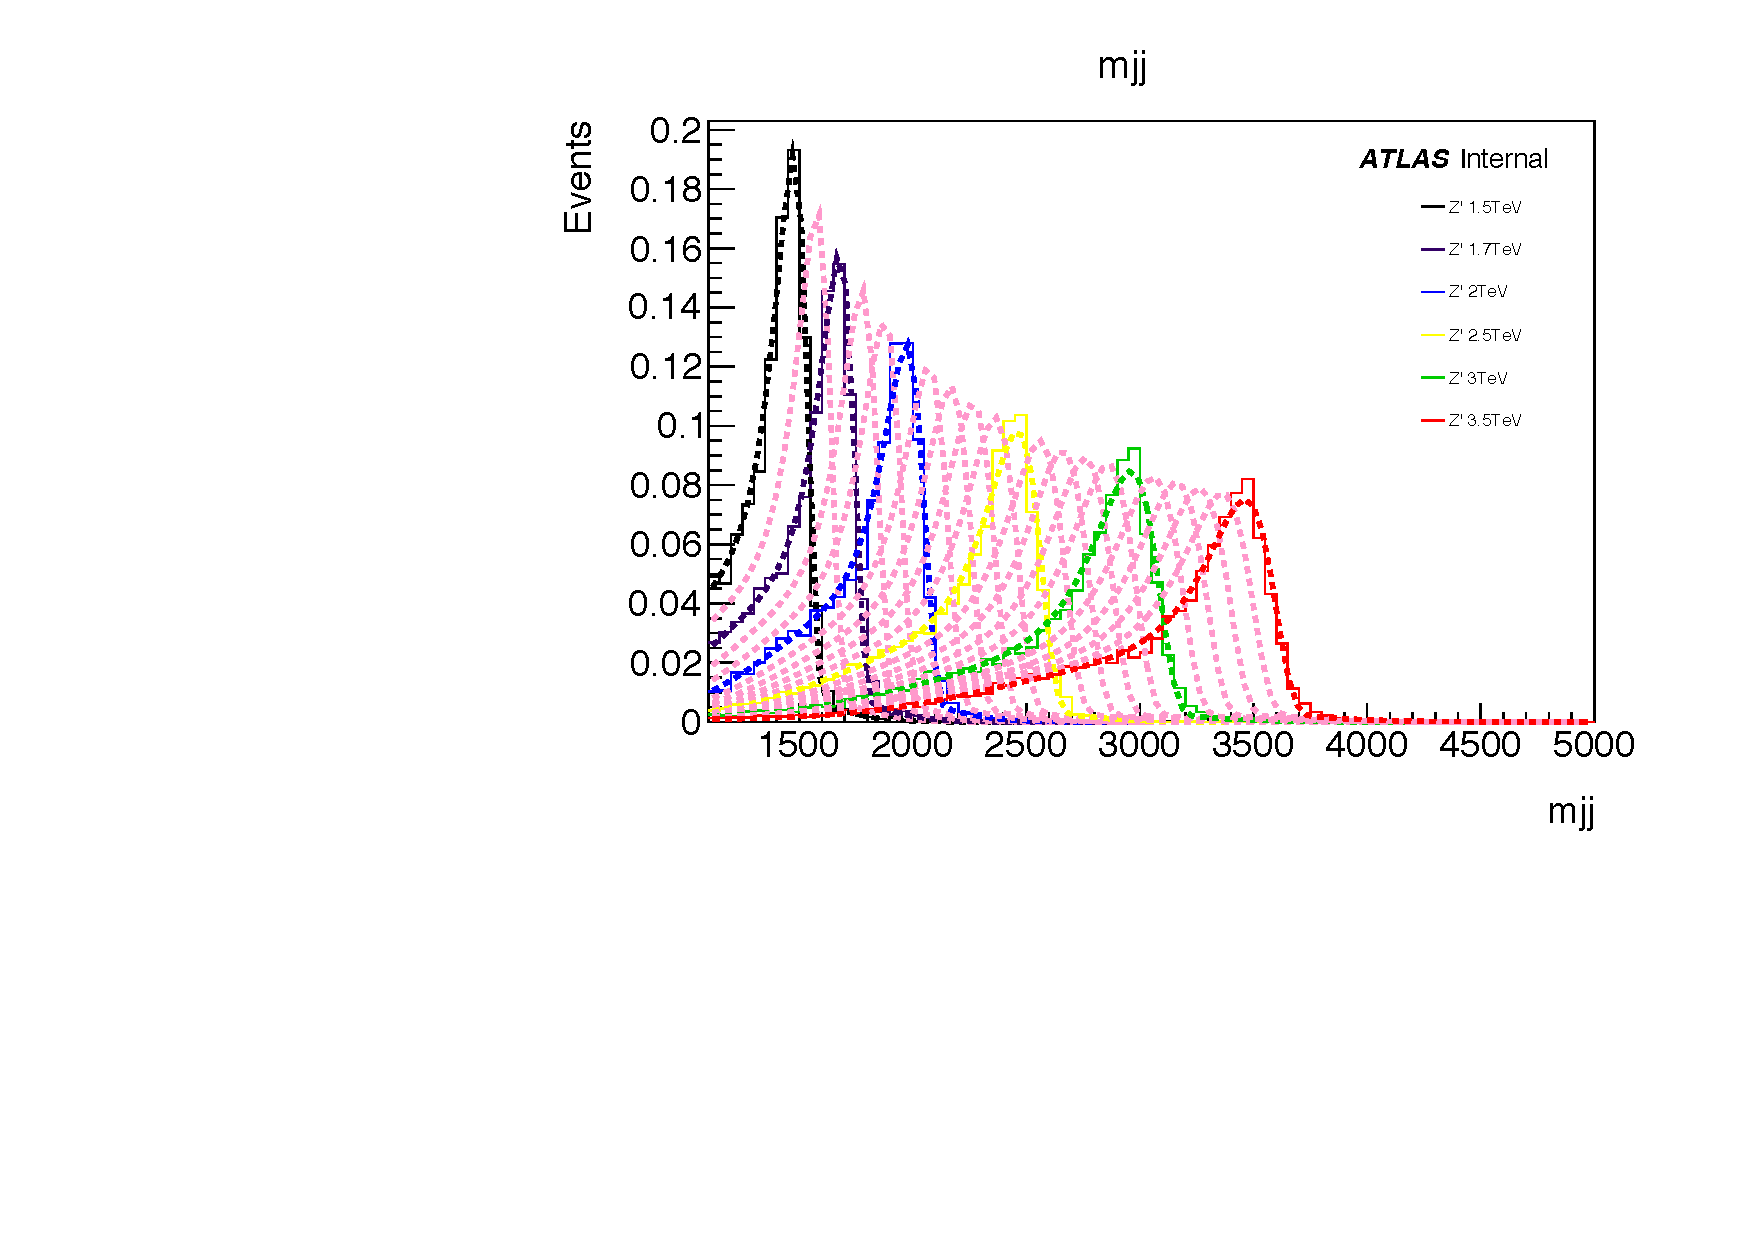
\includegraphics[width=0.48\textwidth]{figures/SWiFt/ZPrime_gSM0p20.pdf} }
	\subfigure[Z' 0.5 SM coupling signals]{ 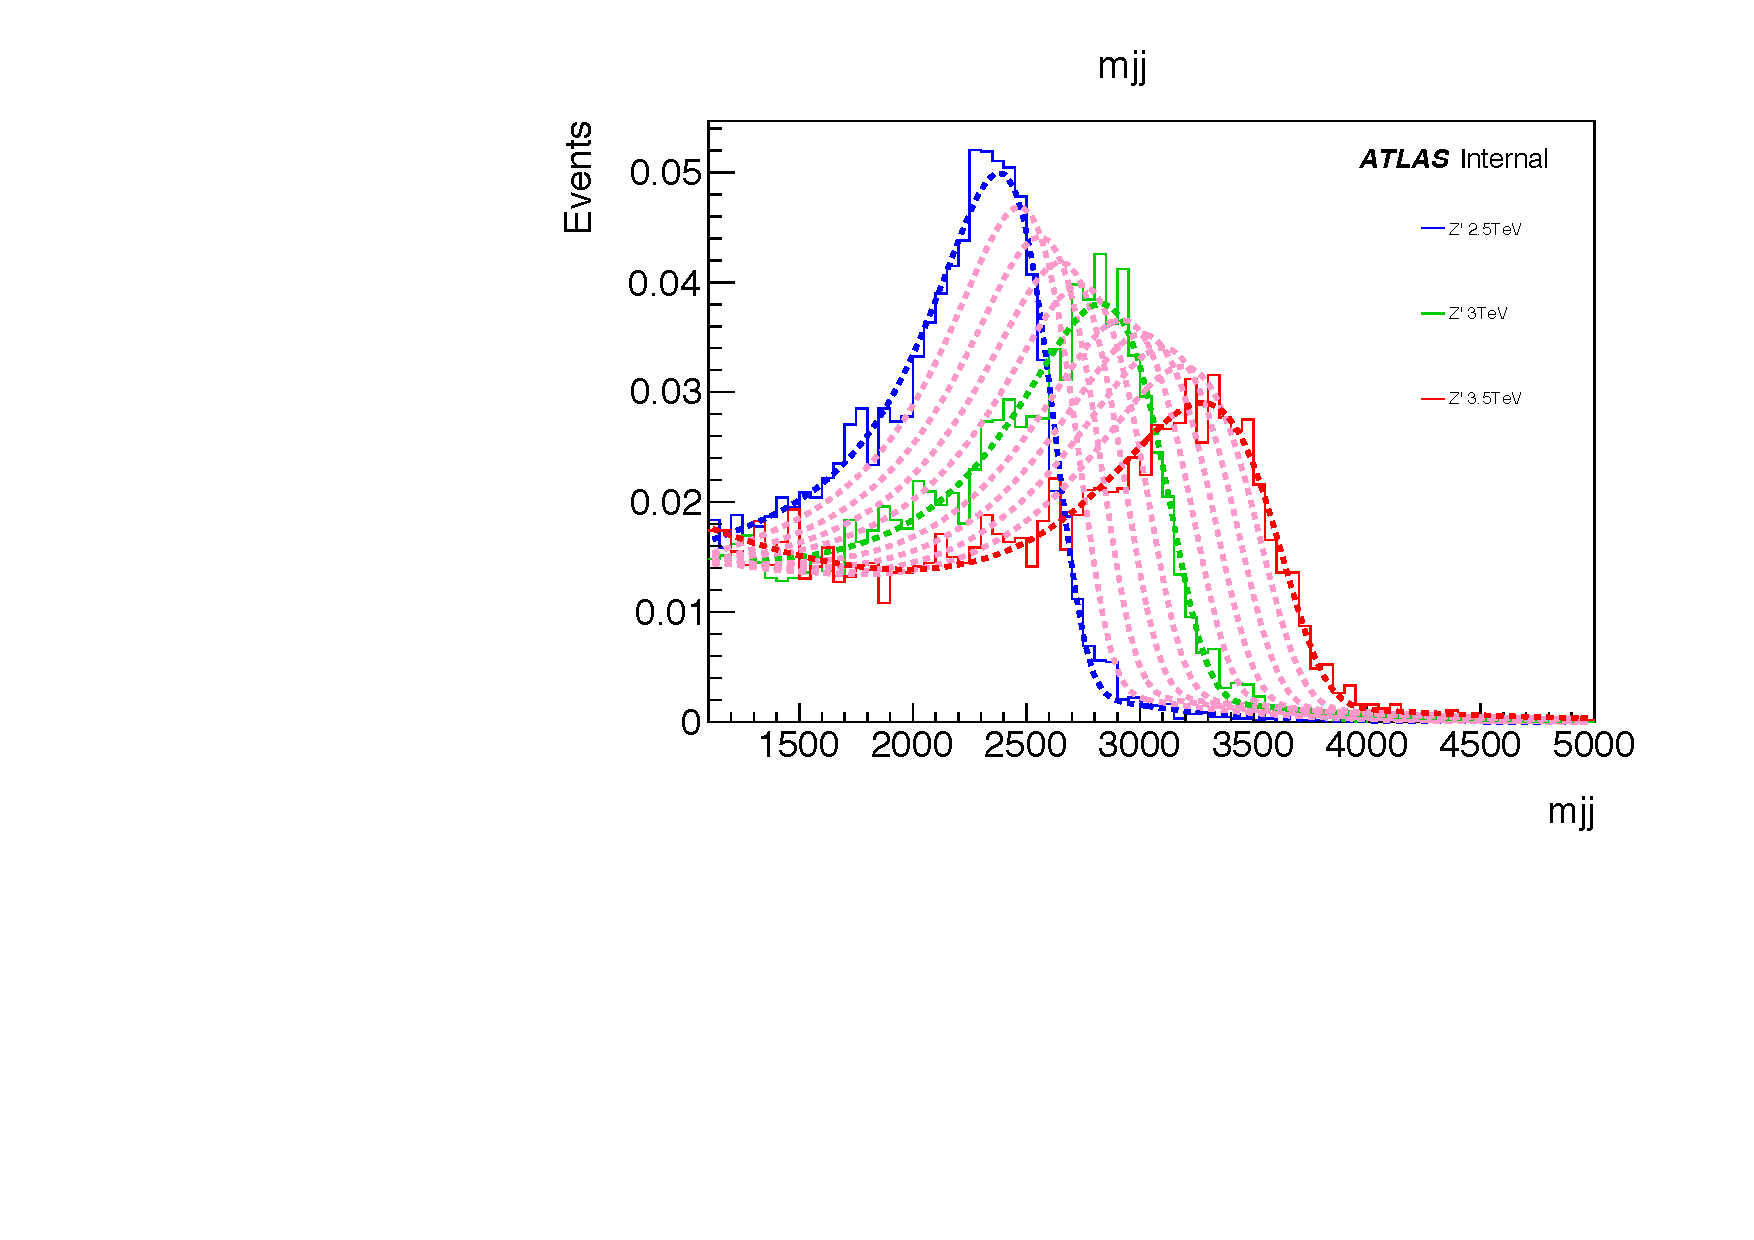
\includegraphics[width=0.48\textwidth]{figures/SWiFt/ZPrime_gSM0p50.pdf} }
	\caption{
		Signal morphing for some MC signals. The solid colored histograms are MC signal shapes and the dotted lines of the same color are fit to the MC shapes. The dotted pink curves are the morphed shapes.  
		\label{fig:morphing}}
\end{figure}

To stress test the morphing technique, tests were done where the a set of mass MC signal shapes were removed and the morphing was done with the remaining shapes. The results of this test is shown in figure~\ref{fig:morphingTest}, where in (a) integer MC q* shapes (2 \TeV\ , 3 \TeV\ , 4 \TeV\ , 5 \TeV\ , 6 \TeV\ ) are removed and morphing is done using the odd shapes only and in (b) fractional MC shapes (2.5 \TeV\ , 3.5 \TeV\ , 4.5 \TeV\ , 5.5 \TeV\ ) are removed and the even shapes are used for morphing. The technique recovers the shapes of the removed signals fairly well.  

\begin{figure}[!htb]
	\centering
	\subfigure[q* signals. Morphing with odd masses only.]{ 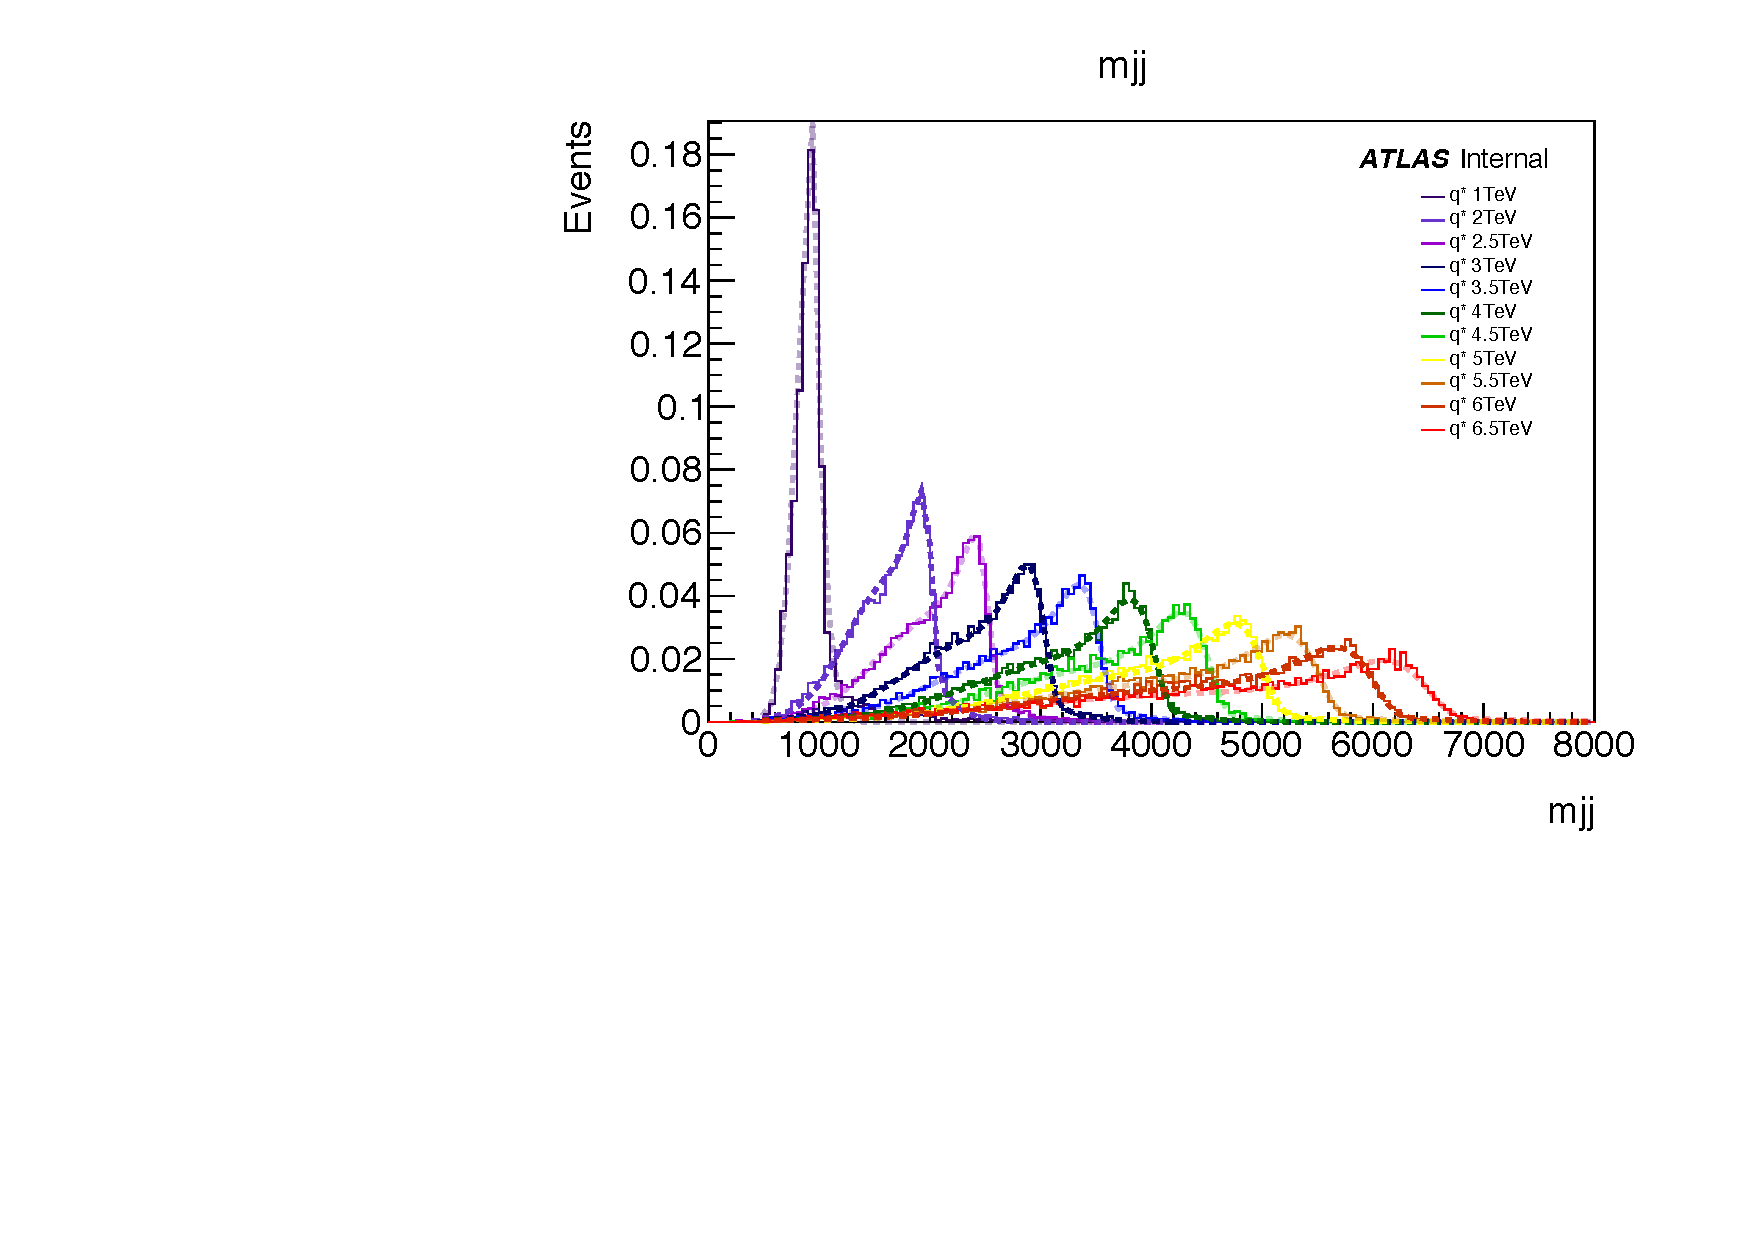
\includegraphics[width=0.48\textwidth]{figures/SWiFt/interpolateWorking_evenRemoved.pdf} }
	\subfigure[q* signals. Morphing with even masses only.]{ 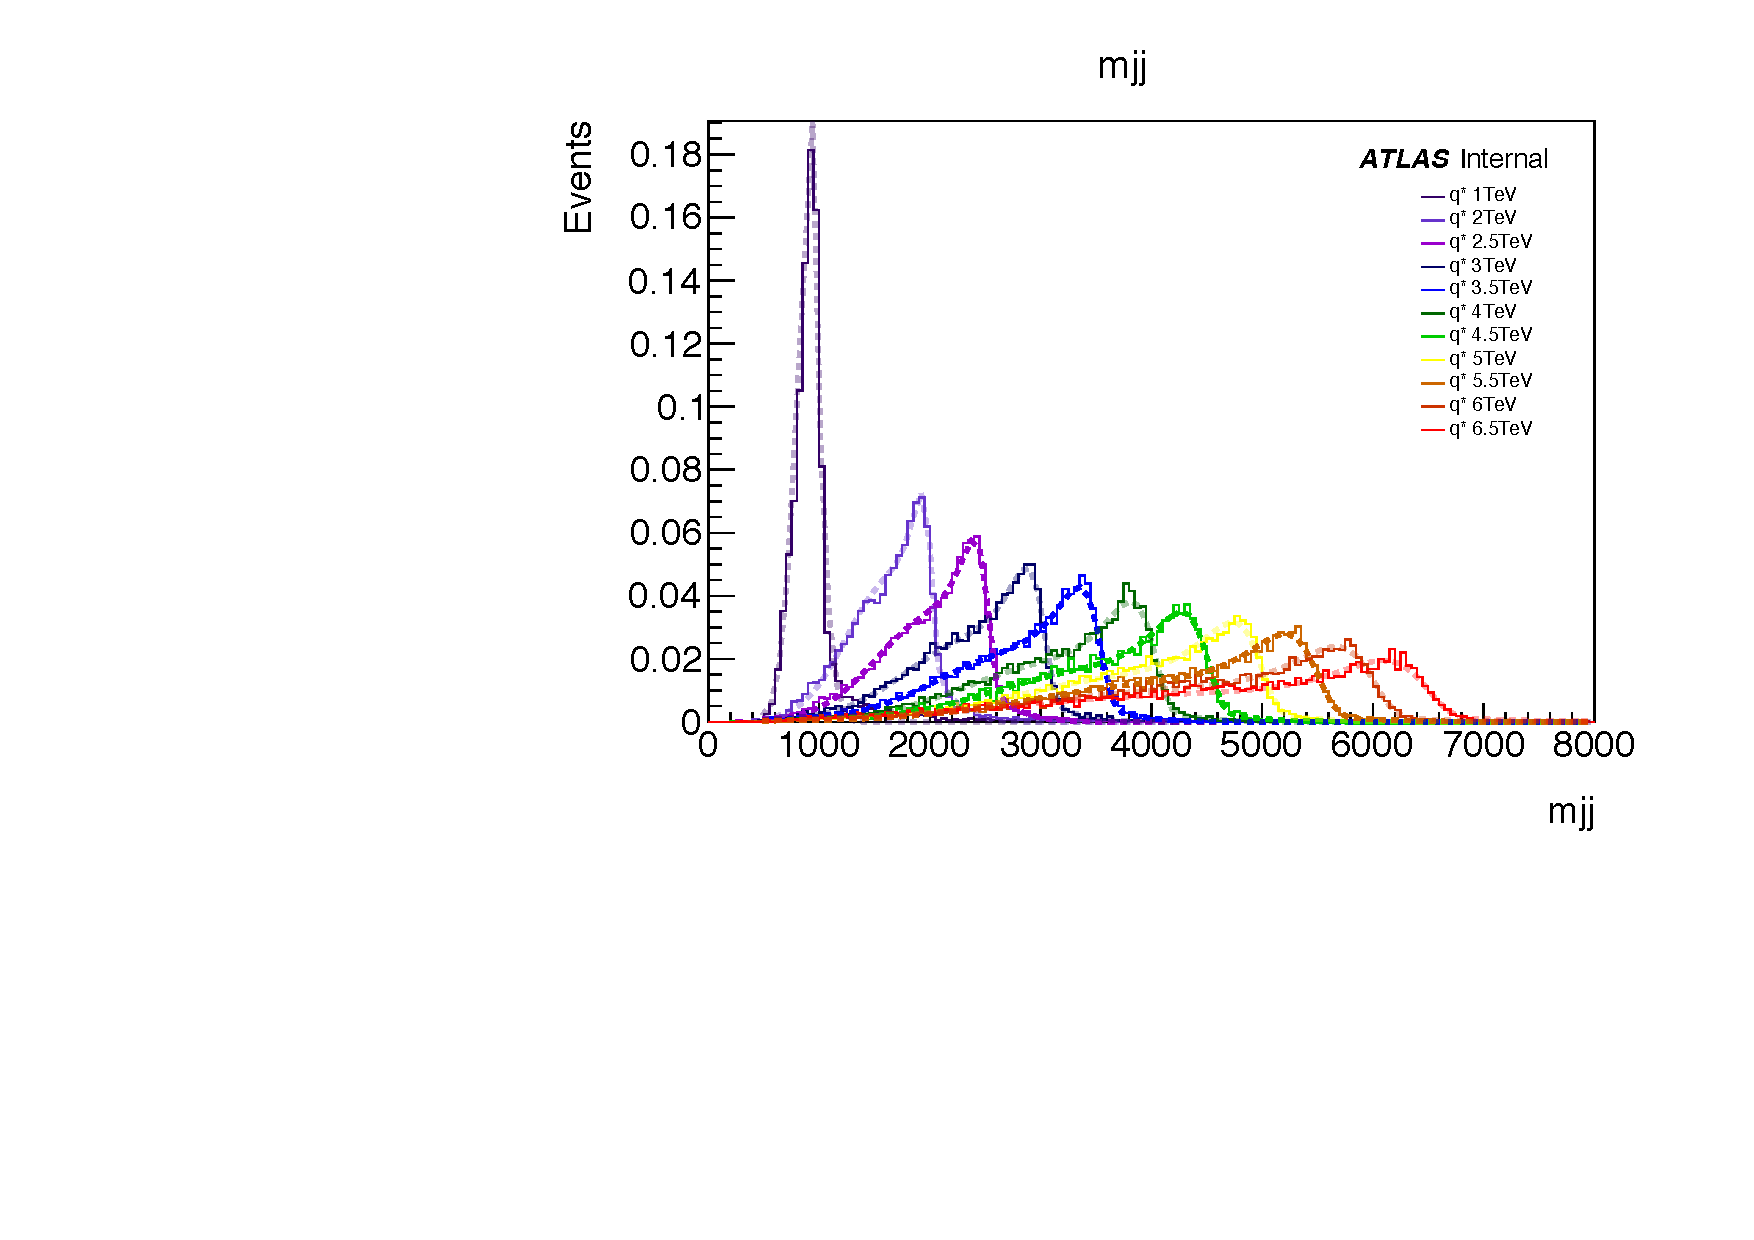
\includegraphics[width=0.48\textwidth]{figures/SWiFt/interpolateWorking_oddRemoved.pdf} }
	\caption{
		Signal morphing stress test. (a) Even mass signals are removed and morphing is done with odd masses only. (b) Odd mass signals are removed and morphing is done with even masses only. 
		\label{fig:morphingTest}}
\end{figure}  



